\documentclass{article}

% hide the (ugly) borders of links
\usepackage[hidelinks]{hyperref}

% no indentation at paragraph, use line break instead
\usepackage[parfill]{parskip}

% math package
\usepackage{amsmath}
\usepackage{amsthm}
\usepackage{amssymb}
\usepackage{mathrsfs}

\usepackage{float}

% custom headers and footers
\usepackage{fancyhdr}

% count page number
\usepackage{lastpage}

% multicolumn
\usepackage{multicol}

% customized margin
\usepackage[top=1in, bottom=1in, left=1in, right=1in]{geometry}

\usepackage{algorithm2e}

\usepackage{graphicx}
\graphicspath{ {figs/} }

% personal info
\newcommand{\id}{Person \texttt{\#}: \texttt{5009 4218}}
\newcommand{\email}{\href{mailto:jinghaos@buffalo.edu}{jinghaos@buffalo.edu}}
\newcommand{\name}{Jinghao Shi}

% cover page
\newcommand{\makecoverpage}{
\maketitle
\thispagestyle{empty}
\newpage
% for double side printing, leave backside of cover page blank
\begin{center}
  \vspace*{\fill}
  \LARGE{\textit{This page intentionally left blank.}}
  \vspace*{\fill}
\end{center}
\thispagestyle{empty}
\newpage
% reset page number counter
\setcounter{page}{1}
}

\newcommand{\problem}[1]{\textbf{Problem.}\quad #1}
\newcommand{\solution}[1]{\textbf{Solution.}\quad #1}
\newcommand{\key}[1]{\textbf{#1}\quad}

\title{\vspace{2in}
CSE589: Modern Network Concepts \\
\vspace{0.5in}
Notes\\
\vspace{3in}
}

\author{
\name\\
\email\\
}

% header and footer
\pagestyle{fancy}
\lhead{\leftmark}
\rhead{CSE589 Notes}
%\rhead{\name\\\email}
\cfoot{\thepage ~/ \pageref{LastPage}}
\renewcommand{\headrulewidth}{0.5pt}

\begin{document}
\makecoverpage

\tableofcontents

\section{Computer Networks and the Internet}

\subsection{Network Edge}
\key{Network edge} Applications and hosts

\subsection{Network Core}
\key{Network core} Routers, Network of networks

\key{Internet protocol stack}
\begin{figure}[H]
  \centering
  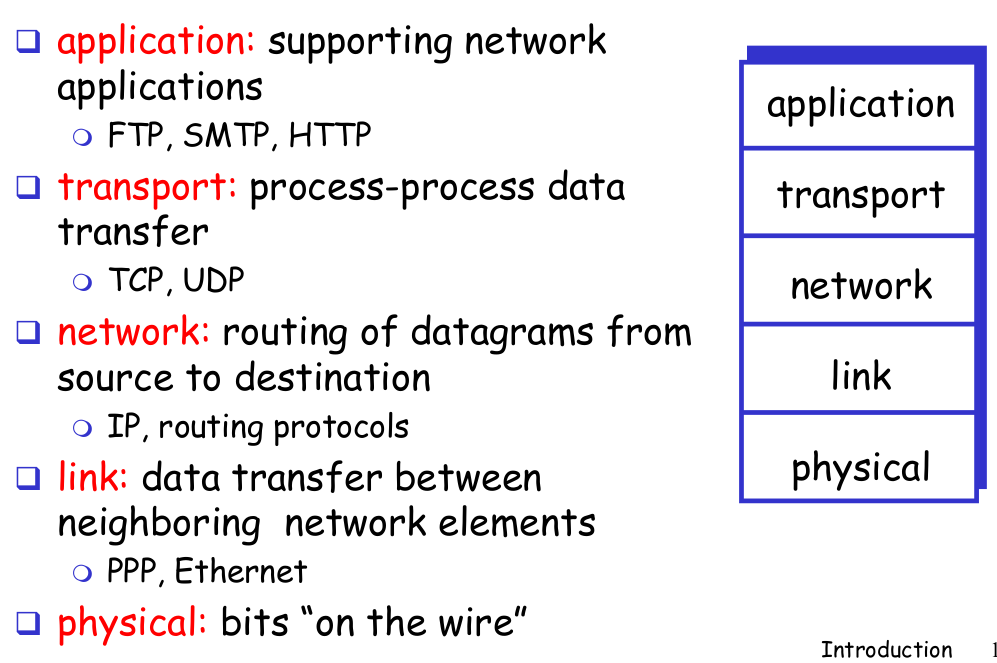
\includegraphics[width=0.5\textwidth]{stack}
\end{figure}

\key{Apps Using TCP} HTTP (Web), FTP (file transfer), Telnet (remote login), SMTP (email)

\key{Apps using UDP} streaming media, teleconferencing, \textbf{DNS}, Internet telephony

\subsection{Delay \& loss in packet-switched networks}

\key{Four sources of delay}
\begin{enumerate}
  \item Transmission delay $d_{\text{trans}}$
  \item Propagation delay $d_{\text{prop}}$
  \item Nodal processing $d_{\text{proc}}$
  \item Queueing $d_{\text{queue}}$
\end{enumerate}
\begin{figure}[H]
  \centering
  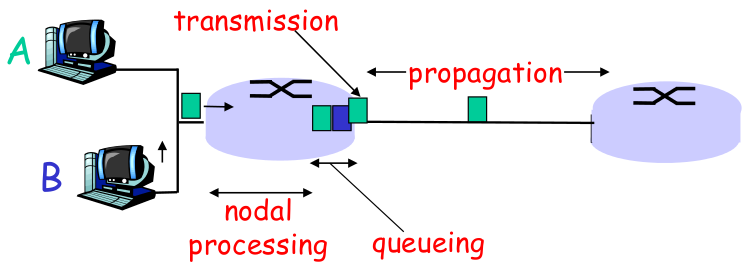
\includegraphics[width=0.5\textwidth]{delay}
\end{figure}

\key{Virtual Circuit} With VC, two packets with the same destination can be assigned two different
VC\# and forced to take different paths.

\section{Application Layer}

\subsection{Principles of network applications}


\key{TCP 4-tuple}
\begin{itemize}
  \item Source $\langle$IP, Port$\rangle$
  \item Dest $\langle$IP, Port$\rangle$
\end{itemize}

\key{What transport service does an app need?}
\begin{figure}[H]
  \centering
  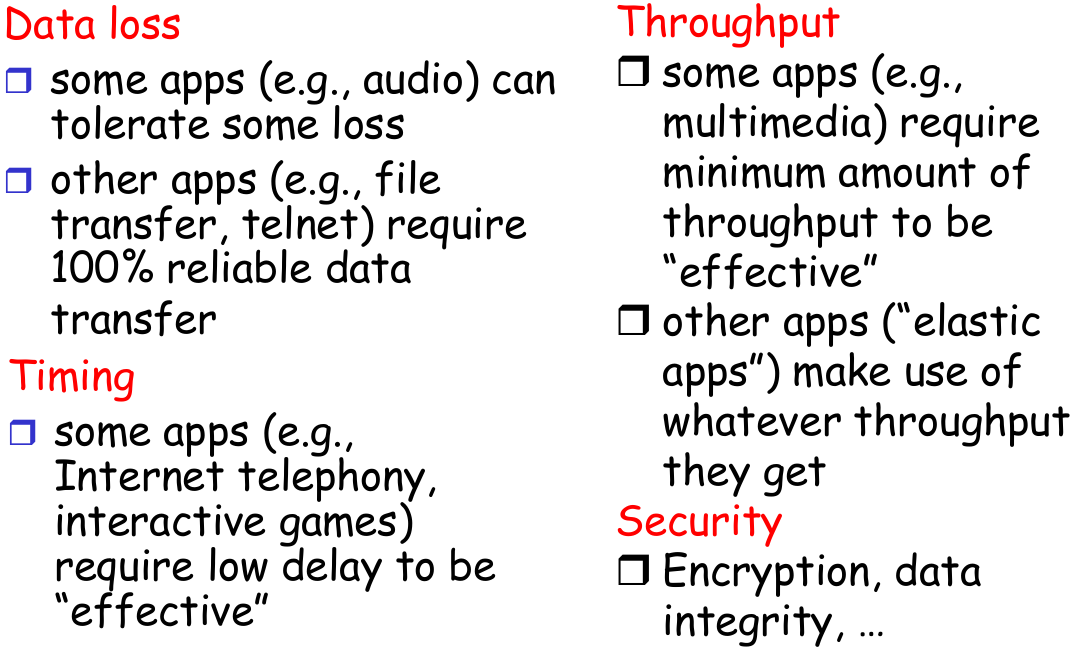
\includegraphics[width=0.5\textwidth]{transport}
\end{figure}

\subsection{Web and HTTP}

\key{HTTP connections}
\begin{figure}[H]
  \centering
  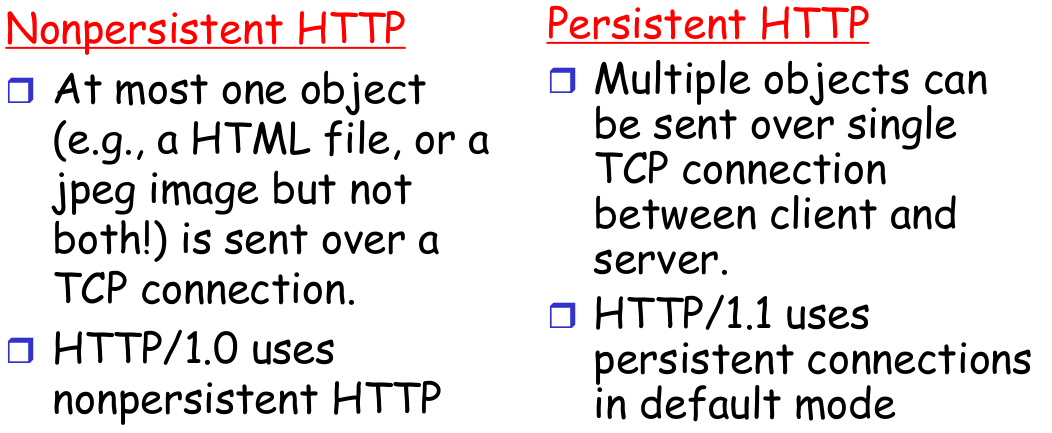
\includegraphics[width=0.5\textwidth]{http_conn}
\end{figure}

\key{Non-Persistent HTTP Response time modeling}
\begin{figure}[H]
  \centering
  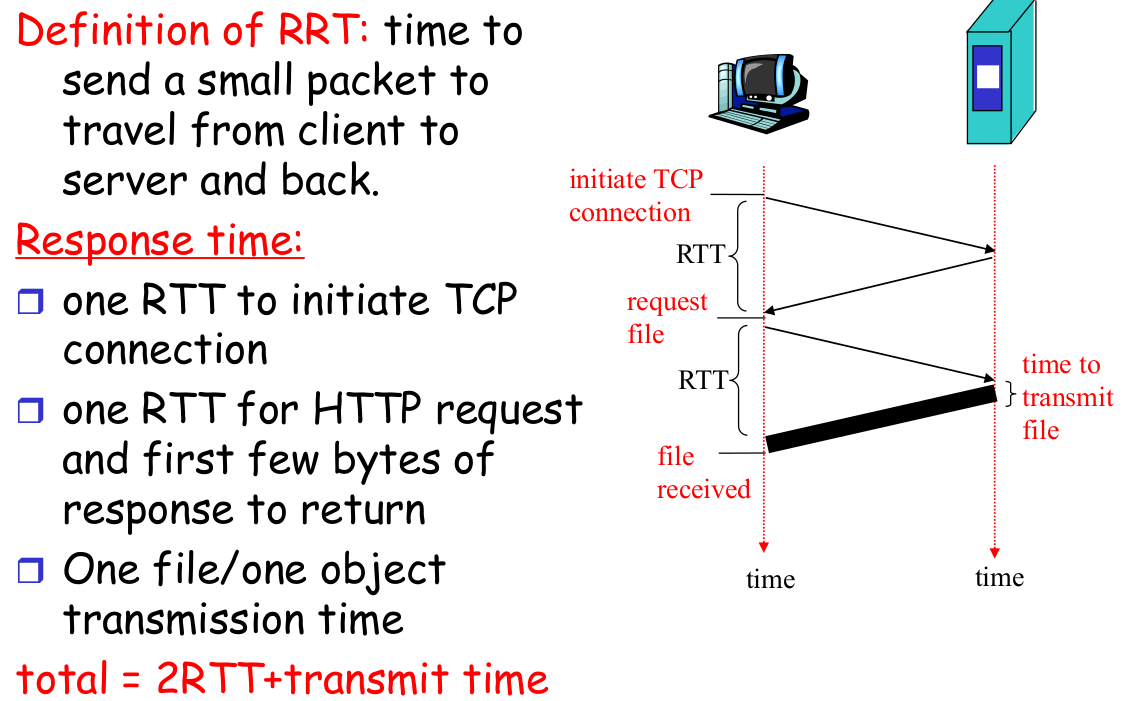
\includegraphics[width=0.5\textwidth]{http}
\end{figure}

\key{Web caches (proxy server) and CDN}
\begin{figure}[H]
  \centering
  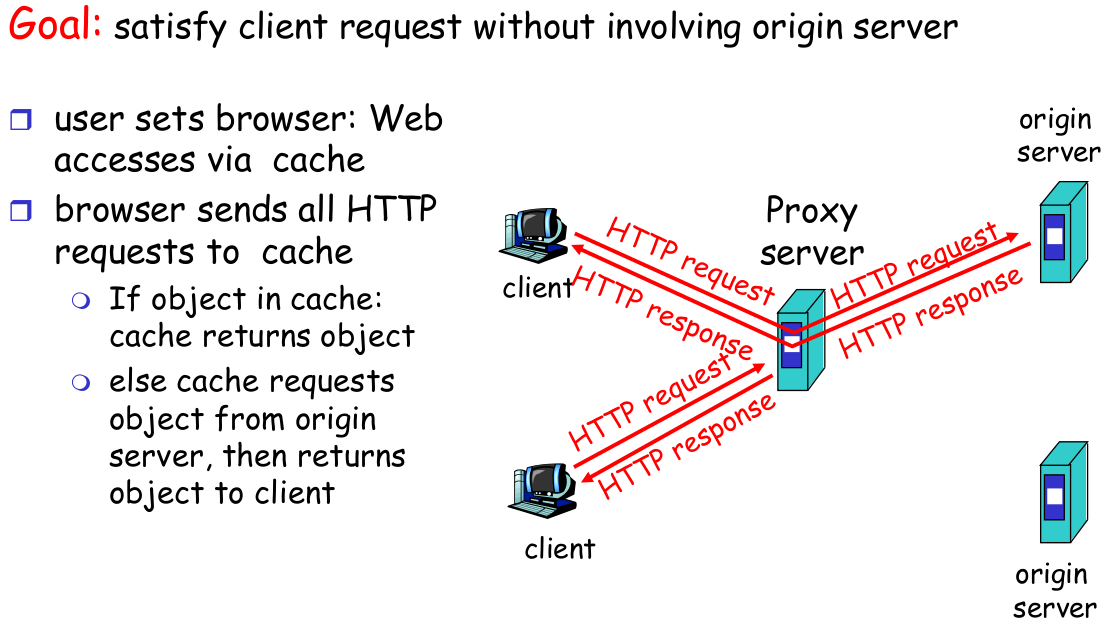
\includegraphics[width=0.48\textwidth]{proxy}
  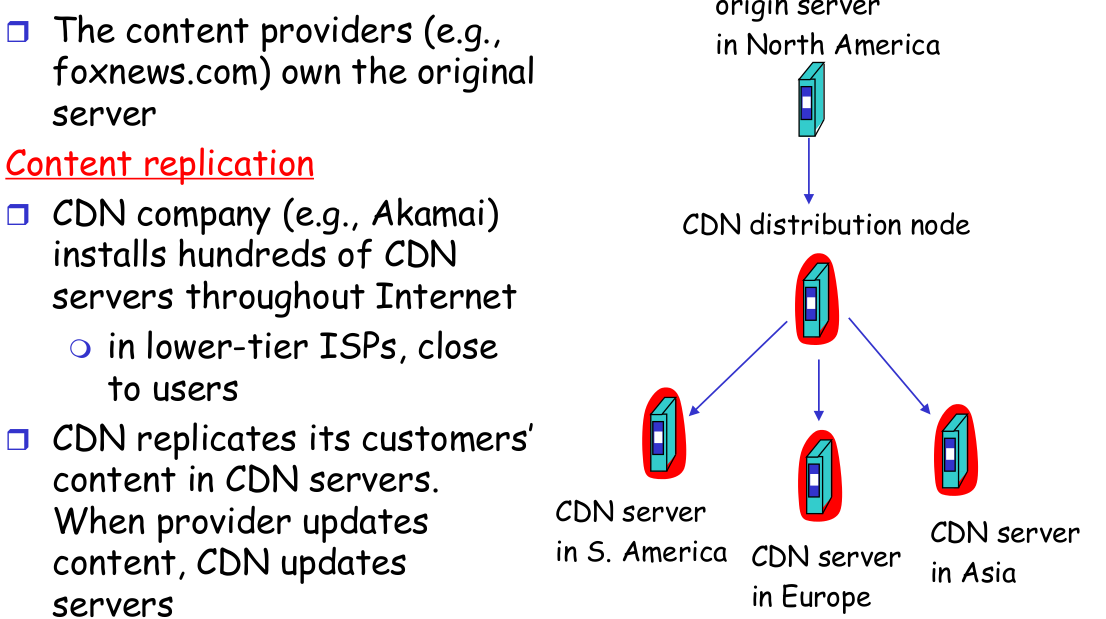
\includegraphics[width=0.48\textwidth]{cdn}
\end{figure}

\subsection{FTP}

\key{FTP: separate control, data connections}
\begin{figure}[H]
  \centering
  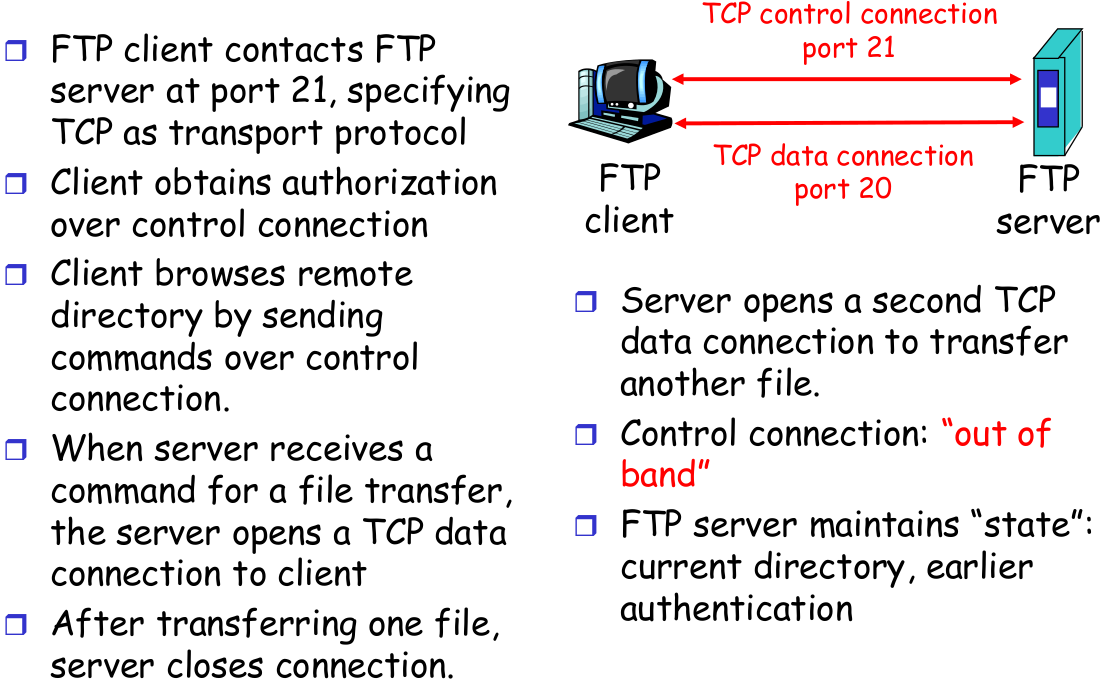
\includegraphics[width=0.48\textwidth]{ftp}
\end{figure}

\subsection{DNS}

\key{DNS: Domain Name System}
\begin{figure}[H]
  \centering
  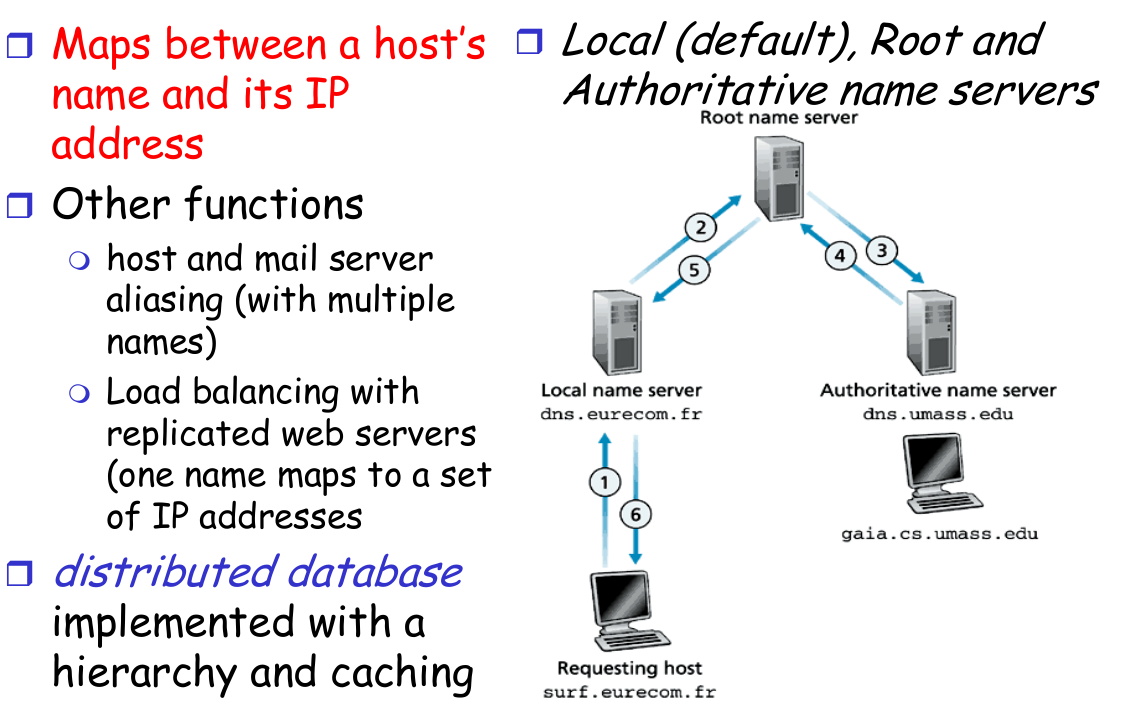
\includegraphics[width=0.48\textwidth]{dns}
\end{figure}


\subsection{P2P applications}

\key{File distribution time: server-client vs. P2P}
\begin{figure}[H]
  \centering
  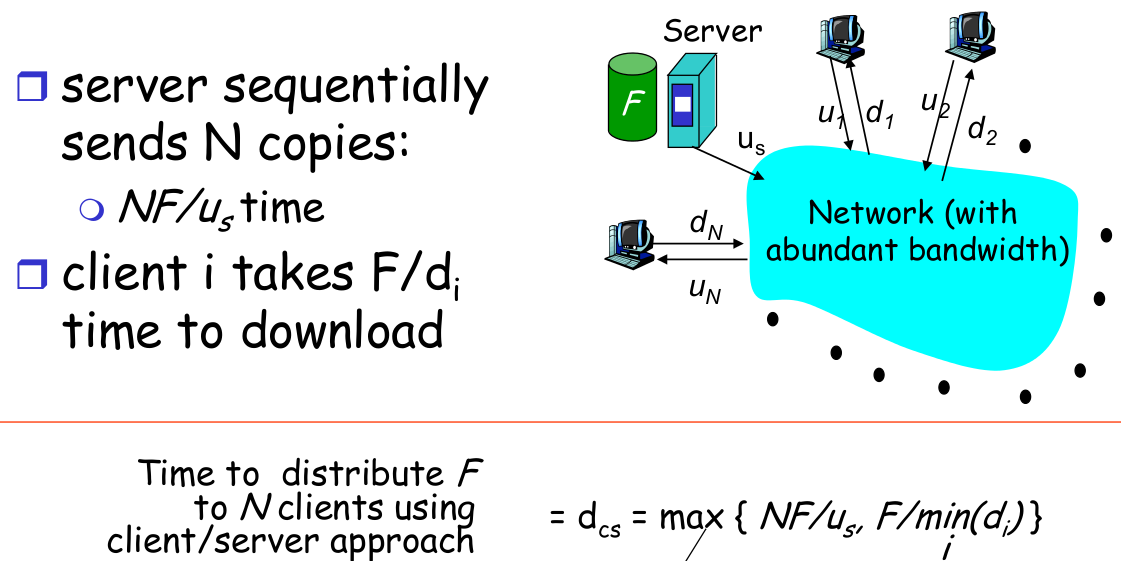
\includegraphics[width=0.48\textwidth]{file-cs}
  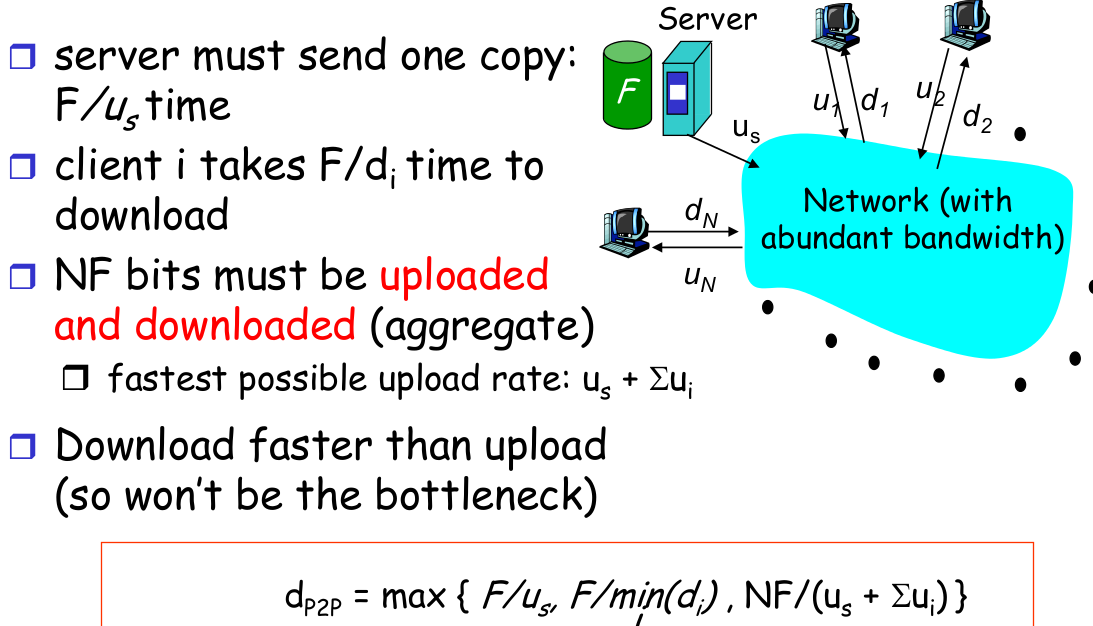
\includegraphics[width=0.48\textwidth]{file-p2p}
\end{figure}

\key{Optimistically Unchoke}
\begin{itemize}
  \item Alice sends chunks to four neighbors currently
    sending her chunks at the highest rate
  \item Re-evaluate top 4 every 10 secs
  \item  Every 30 secs: randomly select another peer, starts sending chunks
  \item Newly chosen peer may join top 4
\end{itemize}



\section{Transport Layer}

\subsection{Transport-layer services}

\key{Internet transport-layer protocols}
\begin{itemize}
  \item Reliable, in-order delivery (TCP)
    \begin{itemize}
      \item congestion control
      \item flow control
      \item connection setup
    \end{itemize}

  \item Unreliable, unordered delivery (UDP)\\
    No-frills extension of ``best-effort'' IP
\end{itemize}

\subsection{Principles of reliable data transfer}

\key{Go-Back-N} Maximum window size is $N-1$
\begin{figure}[H]
  \centering
  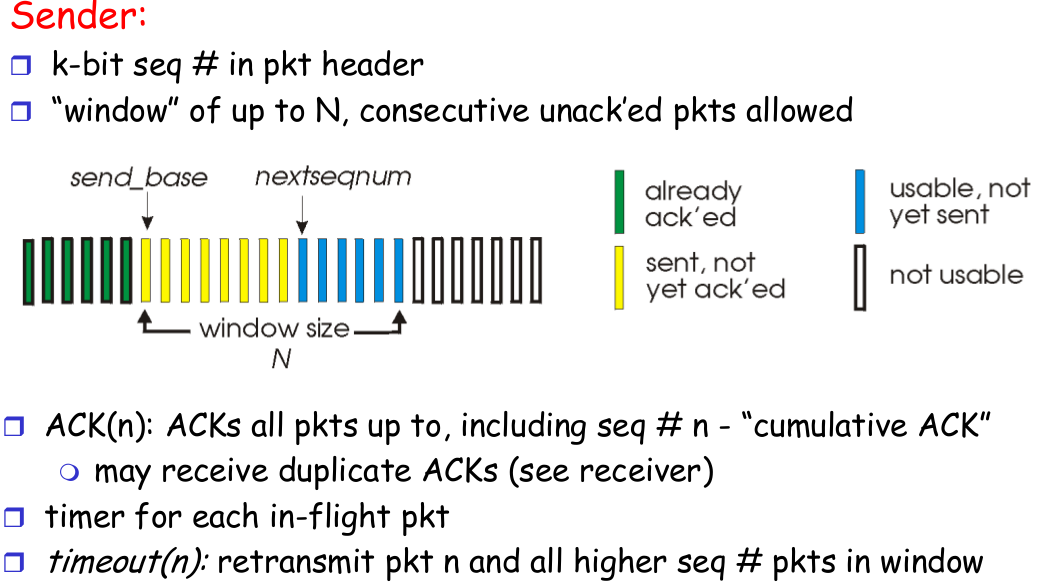
\includegraphics[width=0.48\textwidth]{gbn}
  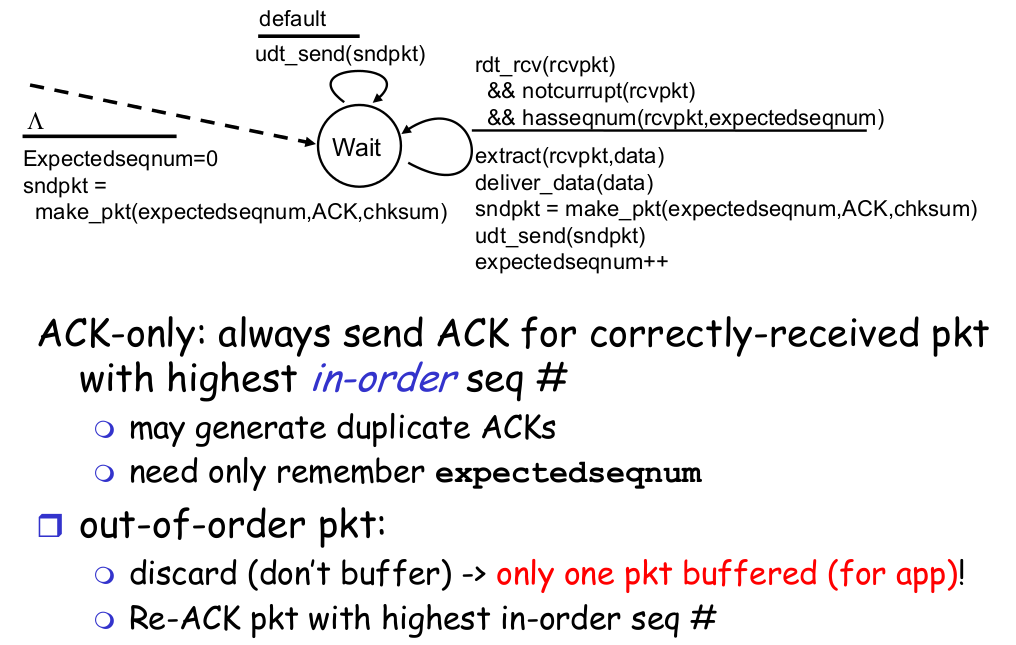
\includegraphics[width=0.48\textwidth]{gbn2}
\end{figure}

\key{Selective Repeat} Maximum window size is $N/2$
\begin{figure}[H]
  \centering
  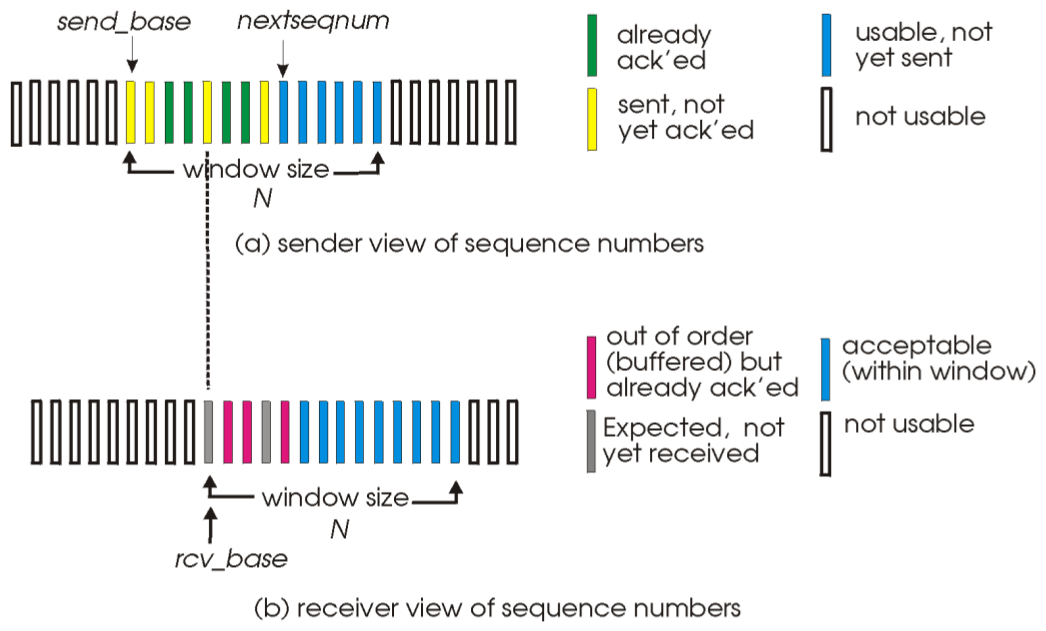
\includegraphics[width=0.48\textwidth]{sr2}
  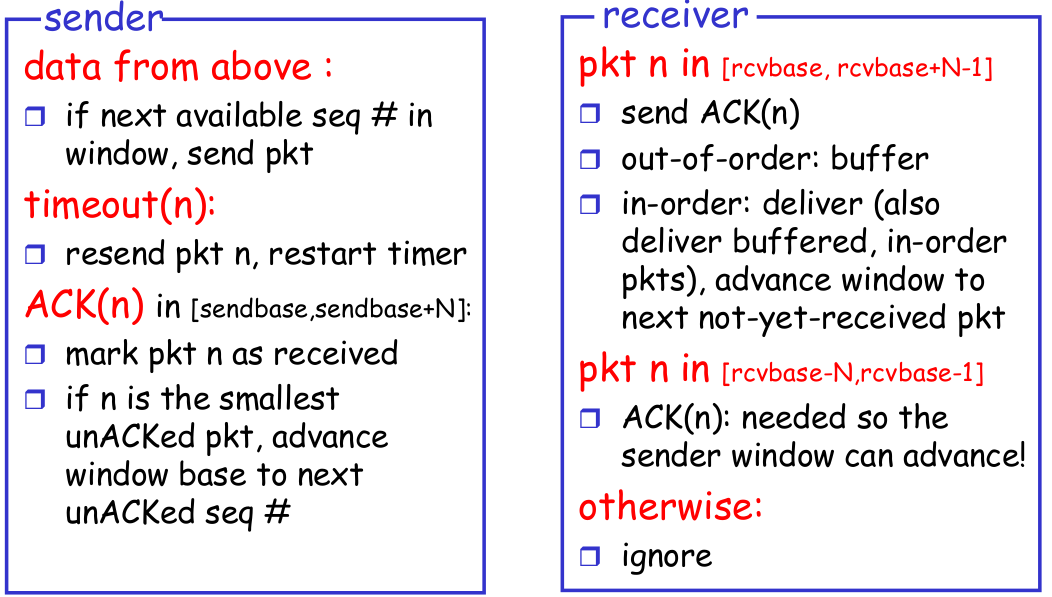
\includegraphics[width=0.48\textwidth]{sr}
\end{figure}

\subsection{Connection-oriented transport: TCP}

\key{TCP segment structure}
\begin{figure}[H]
  \centering
  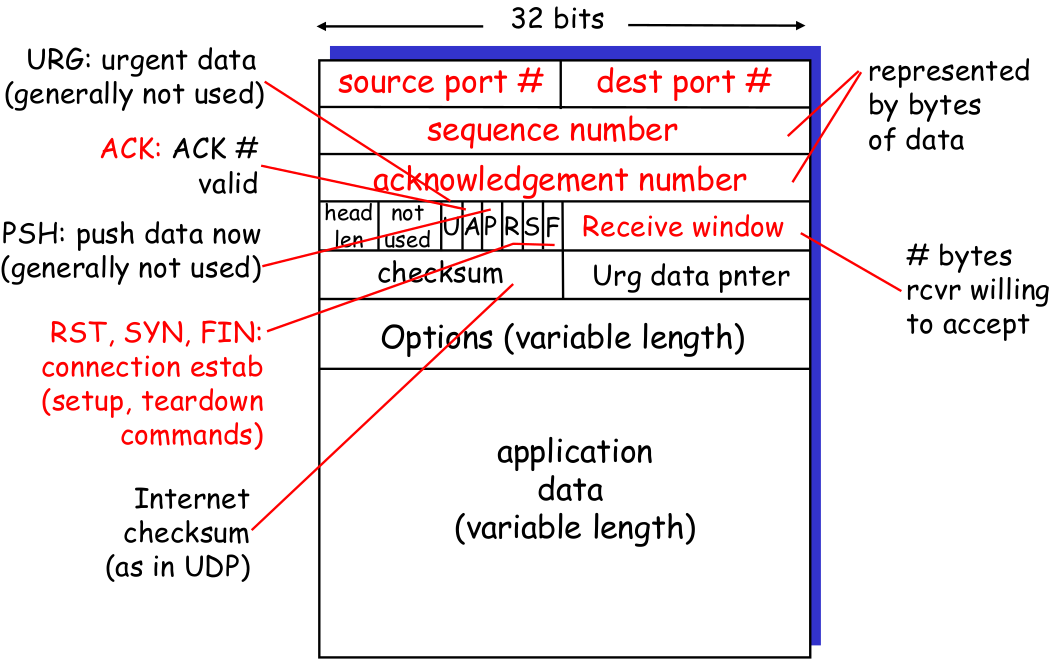
\includegraphics[width=0.48\textwidth]{tcp_frame}
  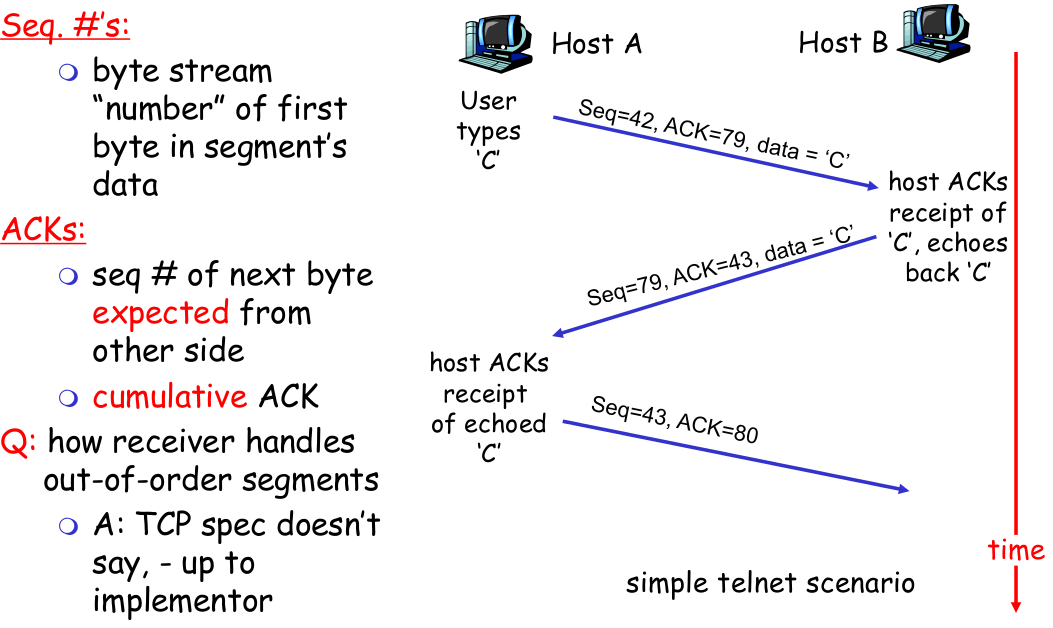
\includegraphics[width=0.48\textwidth]{tcp_seq}
\end{figure}

\key{TCP Connection Establishment (3-way) and Close}
\begin{figure}[H]
  \centering
  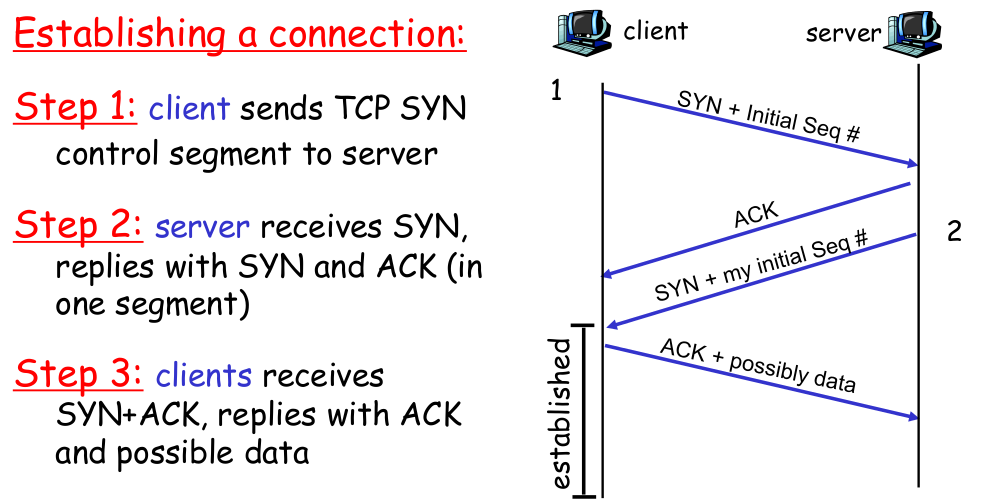
\includegraphics[width=0.48\textwidth]{tcp_conn}
  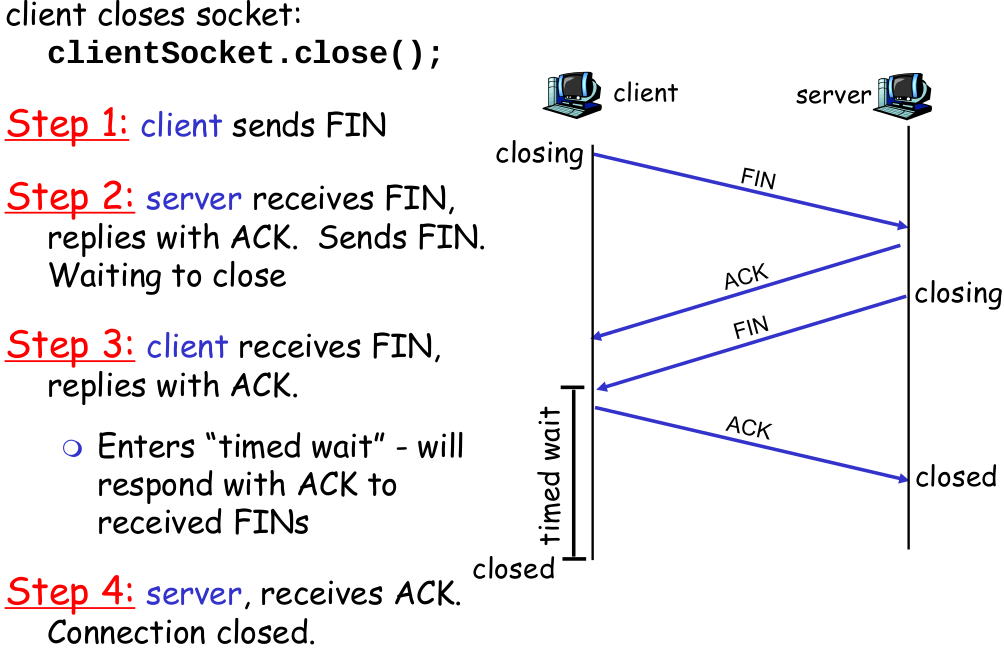
\includegraphics[width=0.48\textwidth]{tcp_close}
\end{figure}

\subsection{TCP congestion control}

\key{Congestion} Too many sources sending too much data too fast for network to handle

\key{TCP AIMD}
\begin{figure}[H]
  \centering
  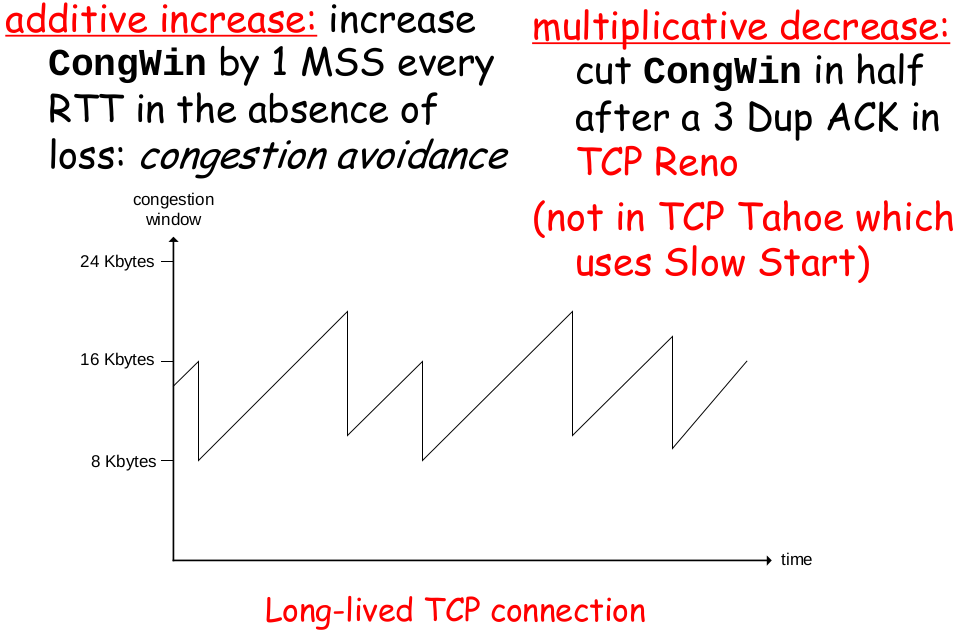
\includegraphics[width=0.5\textwidth]{tcp_aimd}
\end{figure}

\key{Fast Retransmit (Reno)}
\begin{figure}[H]
  \centering
  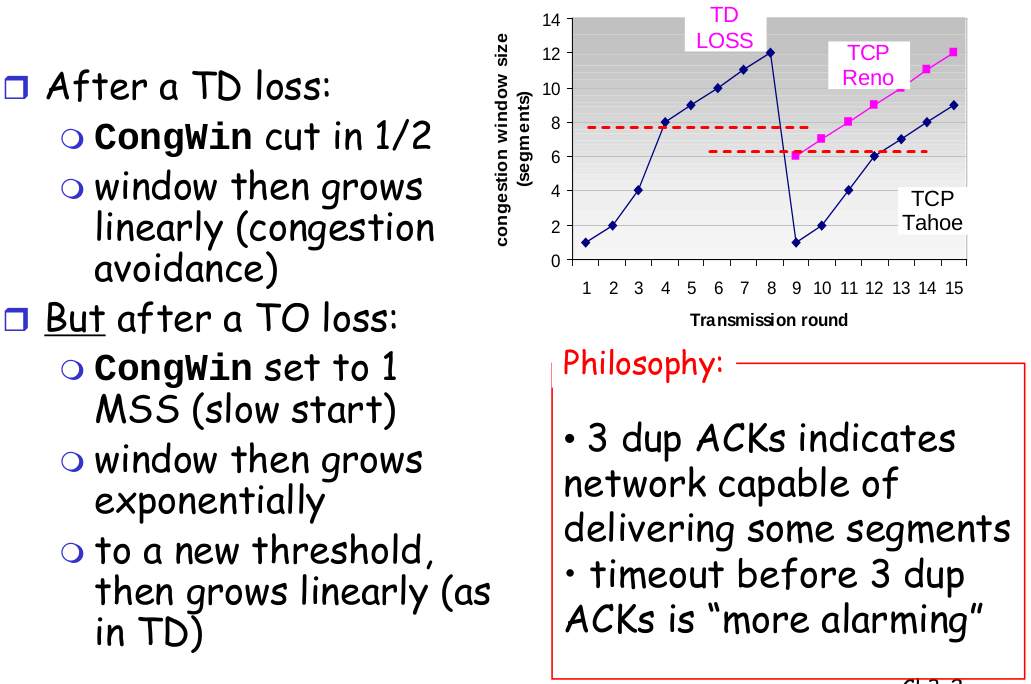
\includegraphics[width=0.48\textwidth]{tcp_reno}
  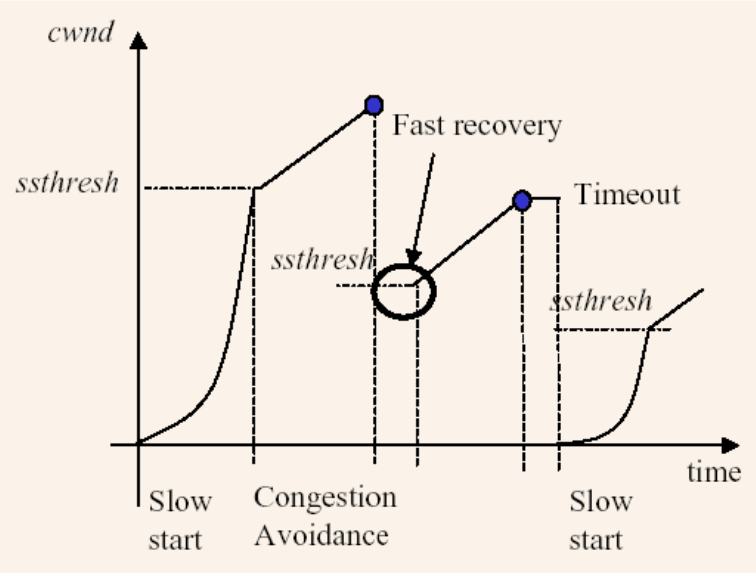
\includegraphics[width=0.48\textwidth]{tcp_phase}
\end{figure}

\key{Why is TCP fair?}
\begin{figure}[H]
  \centering
  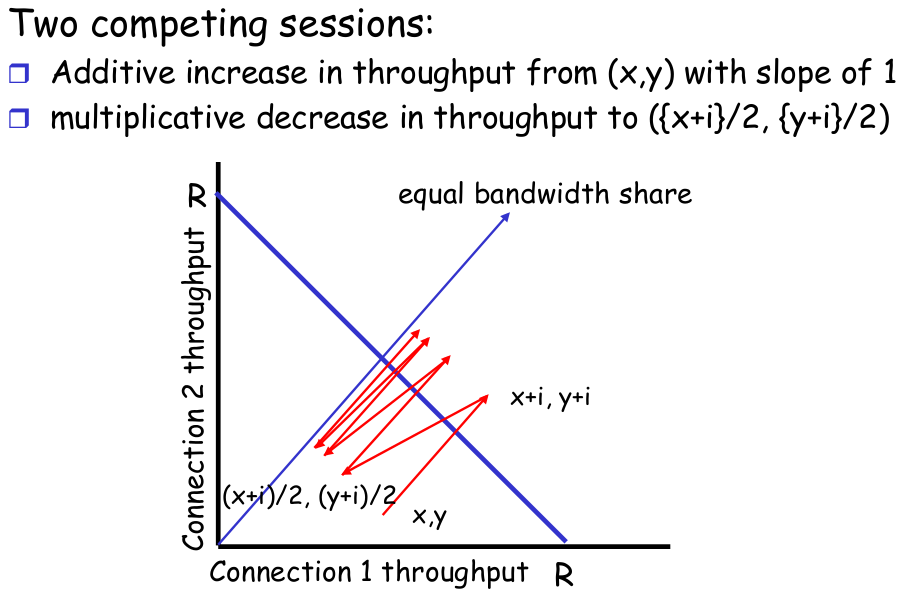
\includegraphics[width=0.5\textwidth]{tcp_fair}
\end{figure}

\key{TCP Delay}
$R$ link rate, $S$ MSS size, $O$ object/file size, $W$ window size
\begin{figure}[H]
  \centering
  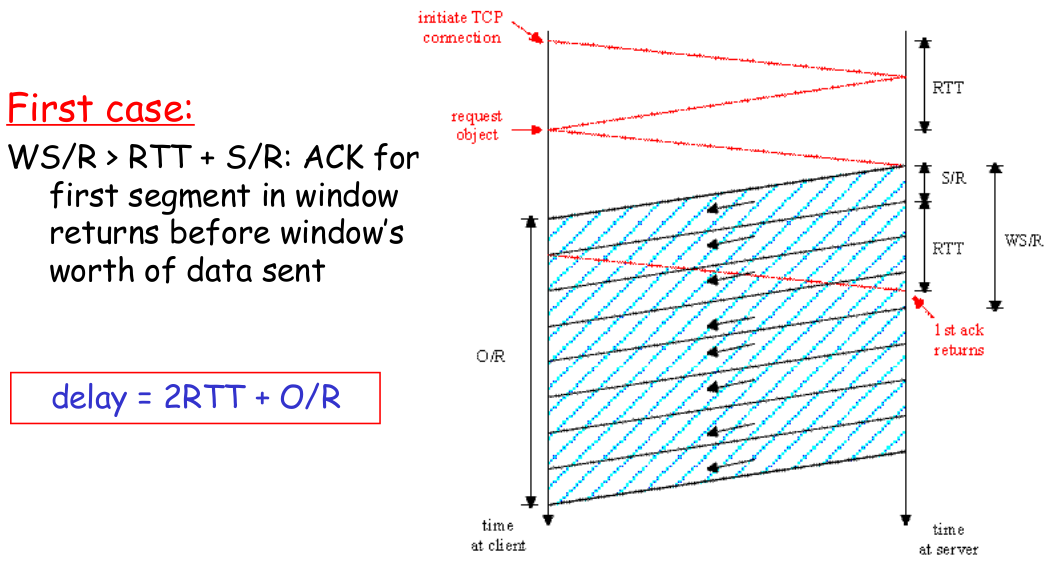
\includegraphics[width=0.48\textwidth]{tcp_delay1}
  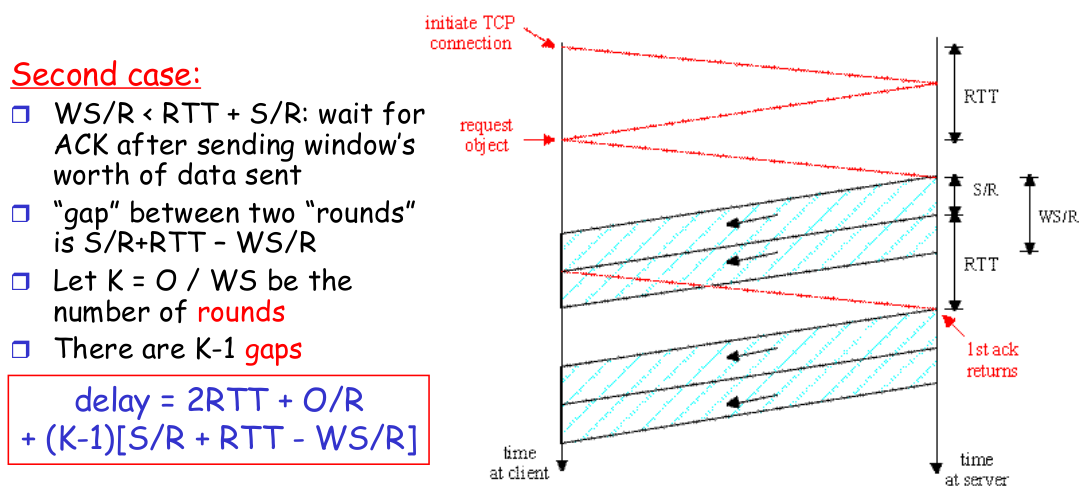
\includegraphics[width=0.48\textwidth]{tcp_delay2}
\end{figure}

\section{Network Layer}

\subsection{Introduction}

\key{Key Network-Layer Functions}
\begin{figure}[H]
  \centering
  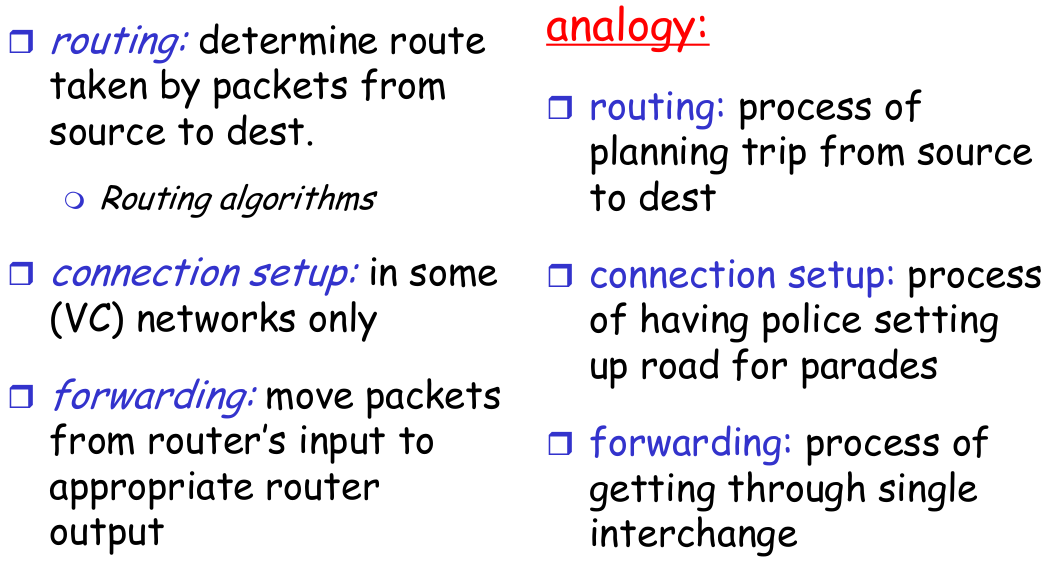
\includegraphics[width=0.48\textwidth]{network_key}
\end{figure}

\subsection{Virtual circuit and datagram networks}

\key{Virtual Circuits vs. Datagram Networks}
\begin{figure}[H]
  \centering
  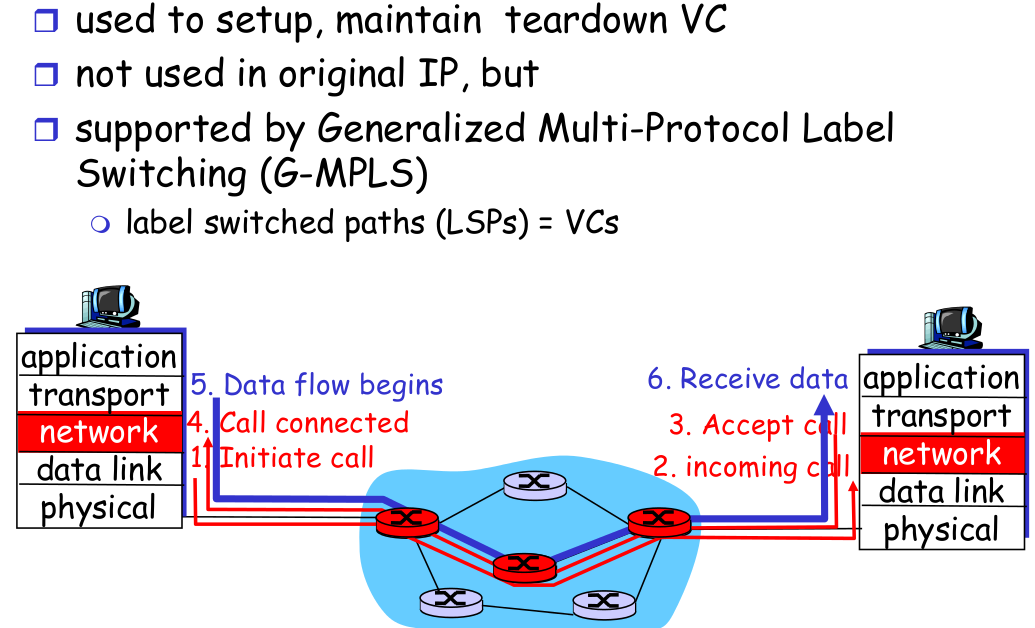
\includegraphics[width=0.48\textwidth]{vc}
  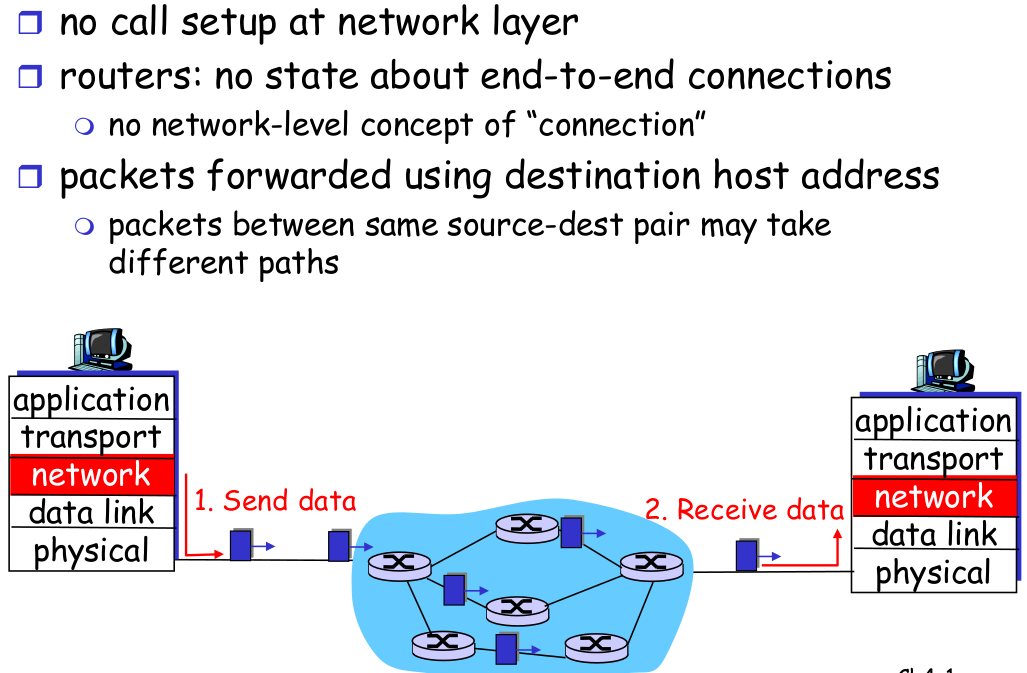
\includegraphics[width=0.48\textwidth]{dg}
\end{figure}

\subsection{IP: Internet Protocol}

\key{IP datagram format}
\begin{figure}[H]
  \centering
  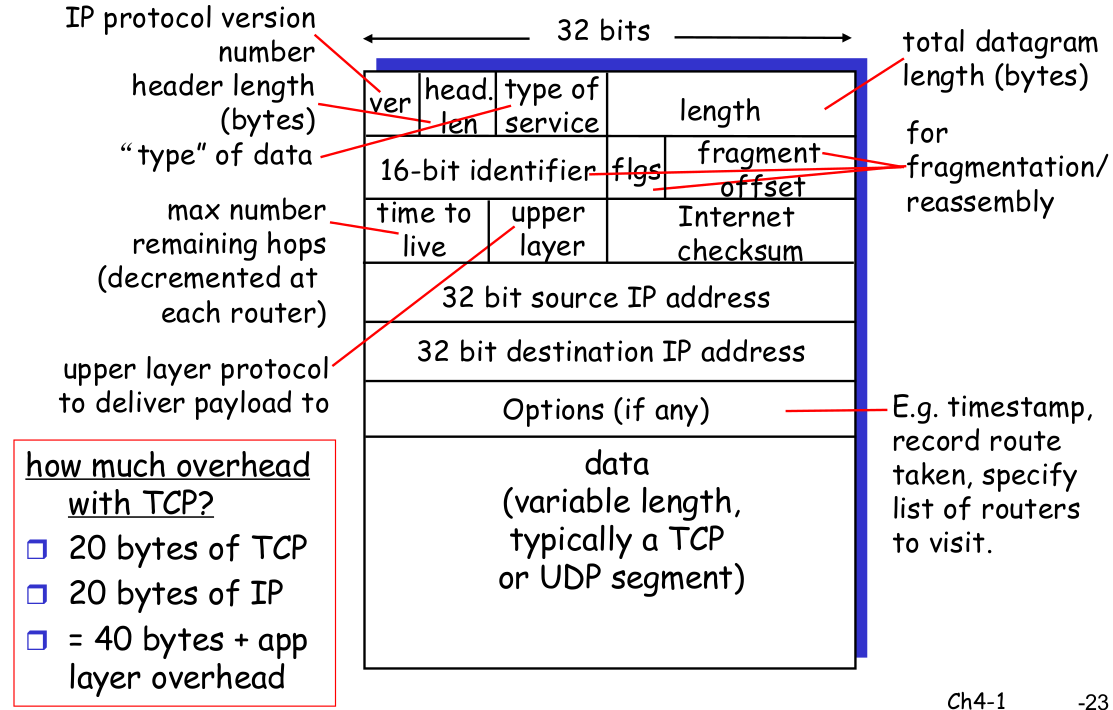
\includegraphics[width=0.48\textwidth]{ip_frame}
  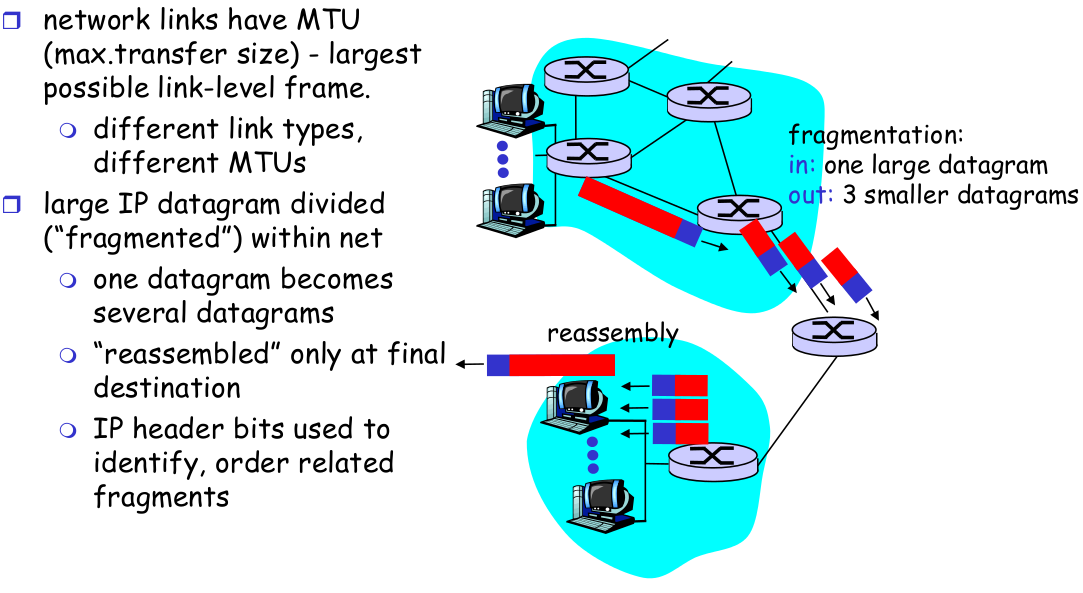
\includegraphics[width=0.48\textwidth]{ip_frag}
\end{figure}

\key{IP addressing: CIDR}
\begin{figure}[H]
  \centering
  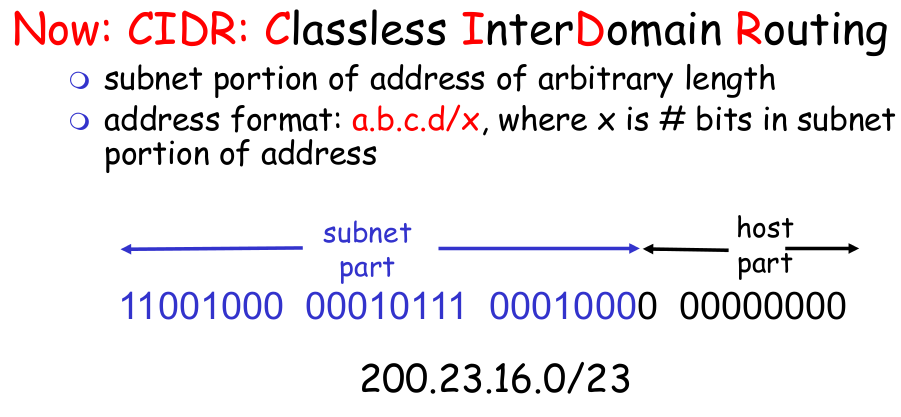
\includegraphics[width=0.5\textwidth]{ip_cidr}
\end{figure}


\key{NAT: Network Address Translation}
\begin{figure}[H]
  \centering
  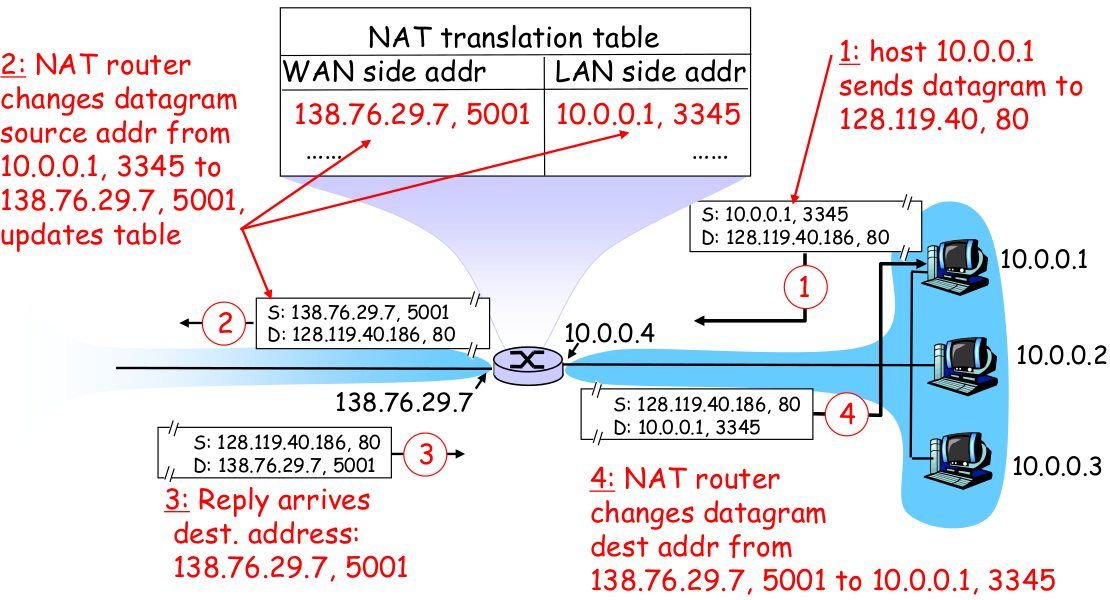
\includegraphics[width=0.48\textwidth]{ip_nat}
  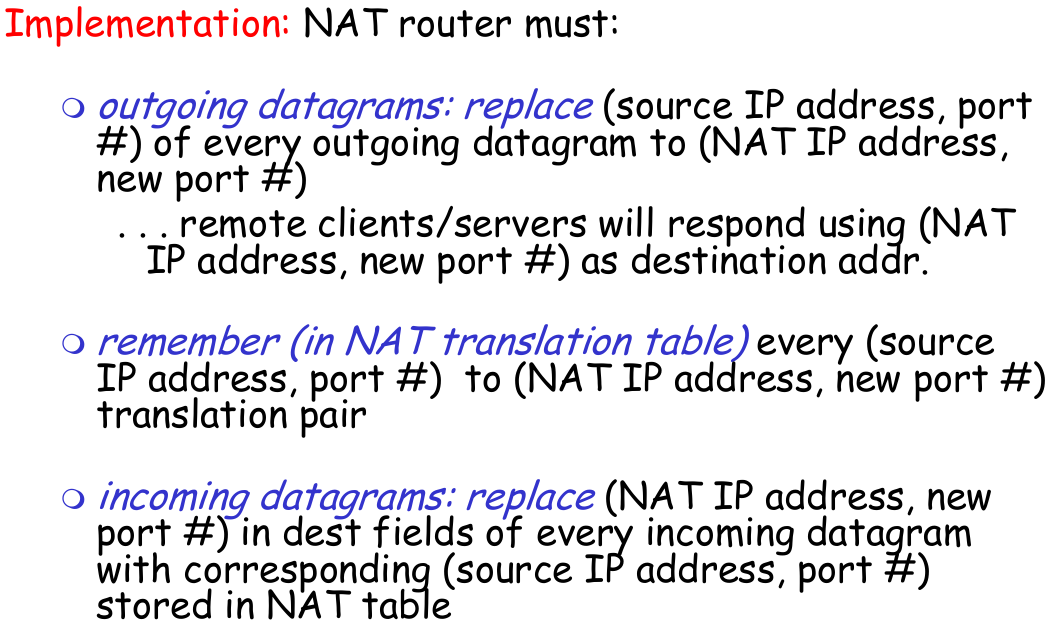
\includegraphics[width=0.48\textwidth]{nat_impl}
\end{figure}

\key{DHCP client-server scenario}
\begin{figure}[H]
  \centering
  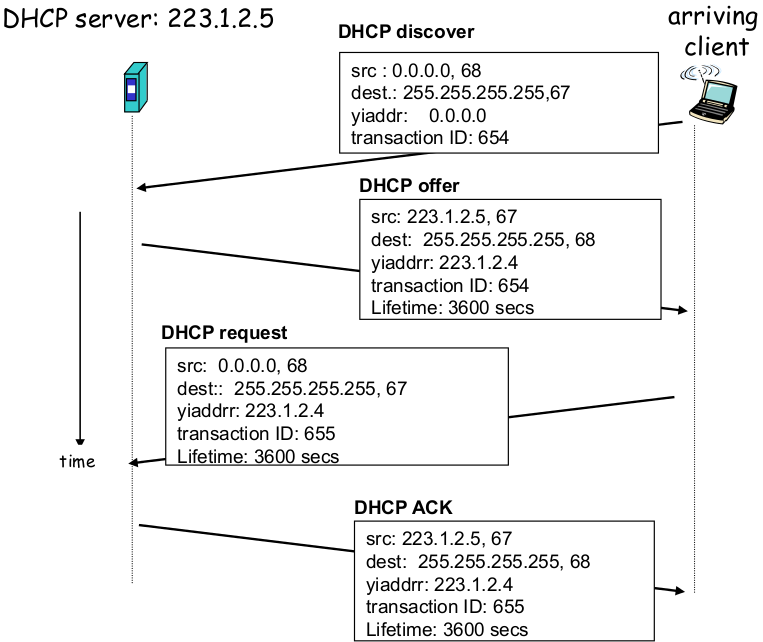
\includegraphics[width=0.48\textwidth]{ip_dhcp}
  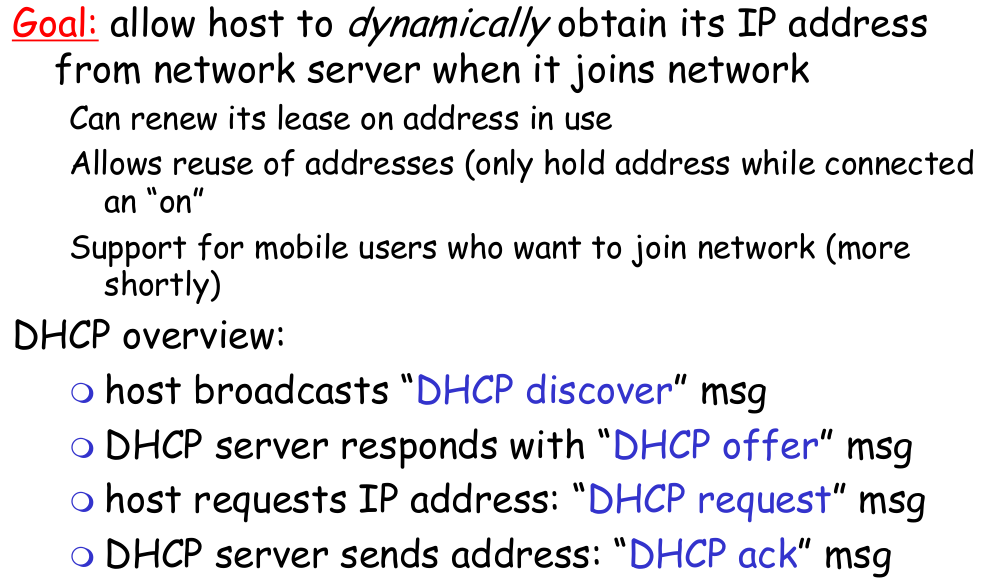
\includegraphics[width=0.48\textwidth]{dhcp_goal}
\end{figure}

Client has to send DHCP request because it probably receive multiple DHCP offers
from different DHCP servers, so that other DHCP servers can know which offer the
client is taking, and can withdraw their offers.

\subsection{Routing algorithms}

\key{Dijkstra algorithm}
\begin{figure}[H]
  \centering
  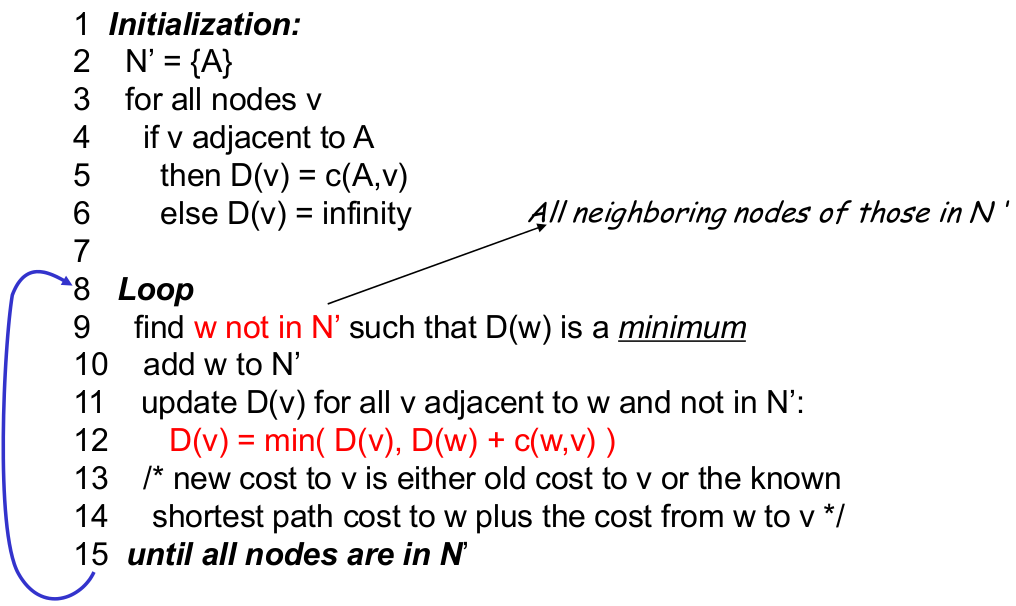
\includegraphics[width=0.49\textwidth]{dijkstra}
  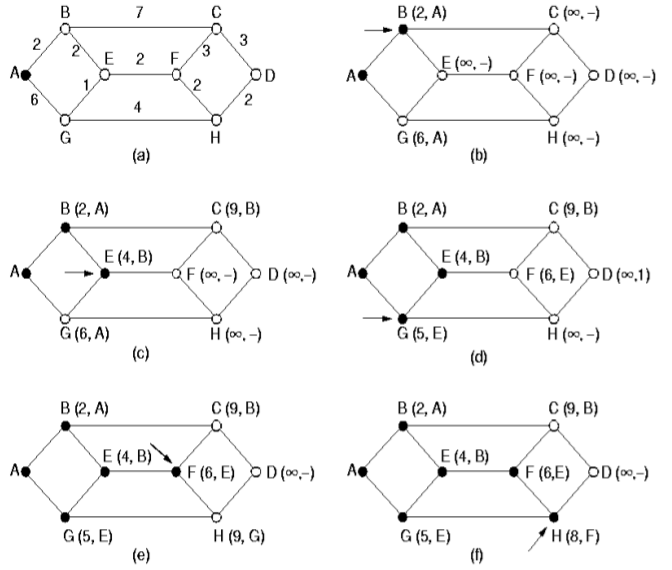
\includegraphics[width=0.49\textwidth]{dijkstra_example}
\end{figure}

\key{Distance Vector}
\begin{figure}[H]
  \centering
  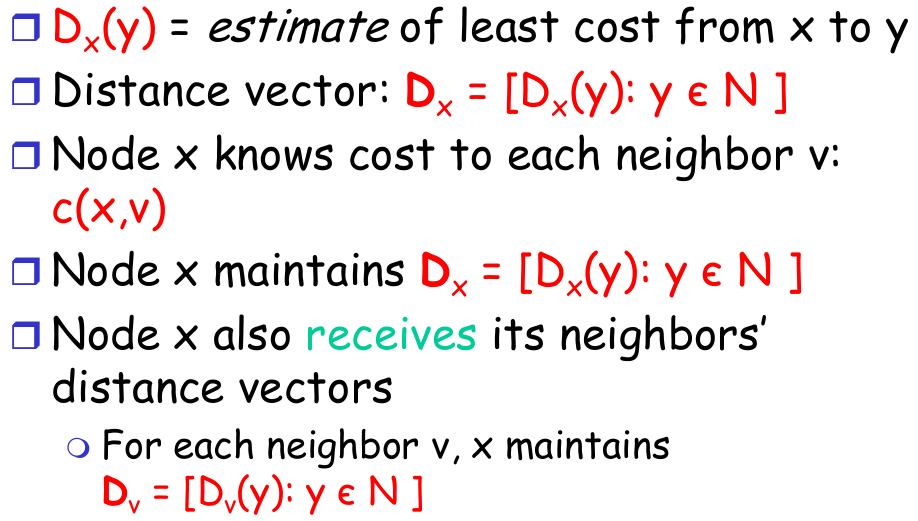
\includegraphics[width=0.49\textwidth]{dv1}
  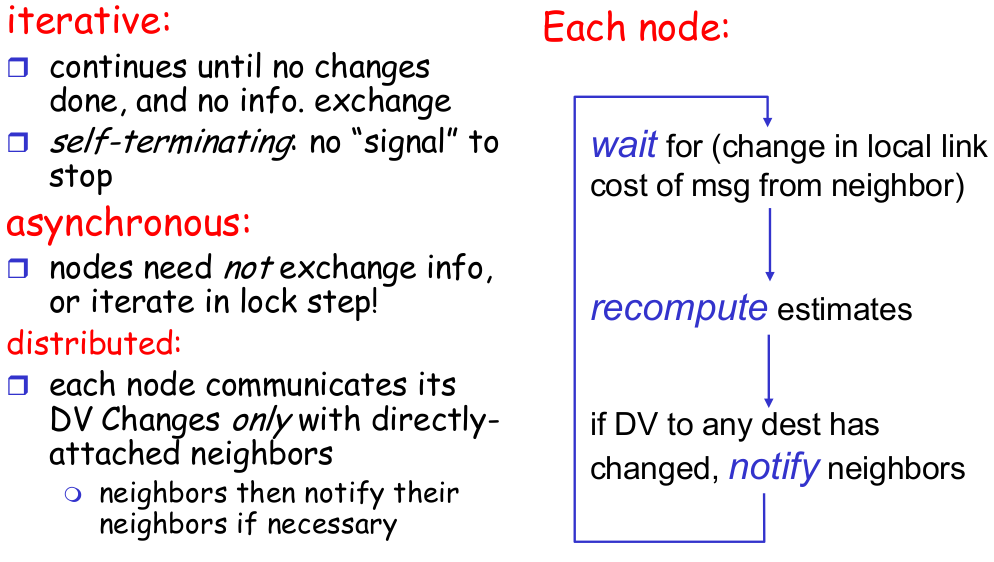
\includegraphics[width=0.49\textwidth]{dv2}
\end{figure}



\key{Hierarchical Routing}
\begin{figure}[H]
  \centering
  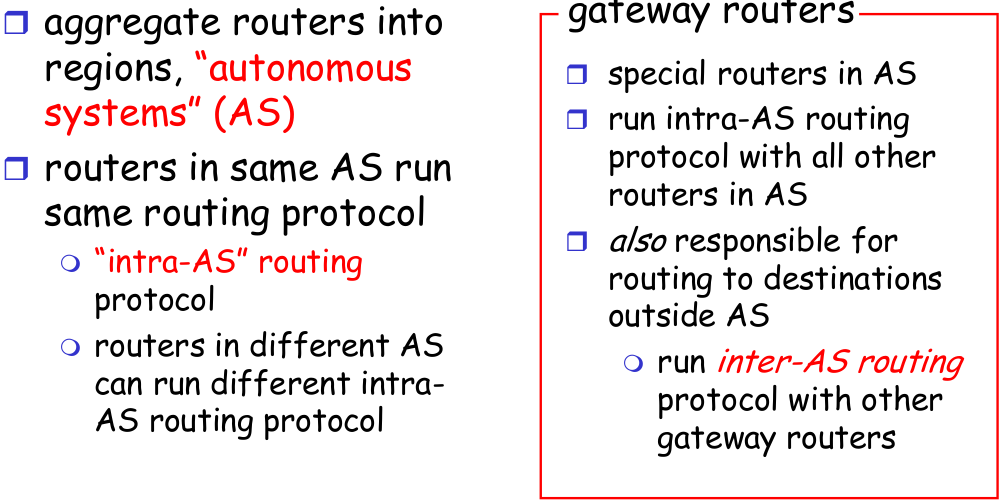
\includegraphics[width=0.5\textwidth]{ip_hierarchy}
\end{figure}

\subsection{Routing in the Internet}

\key{Intra-AS and inter-AS Routing}
\begin{figure}[H]
  \centering
  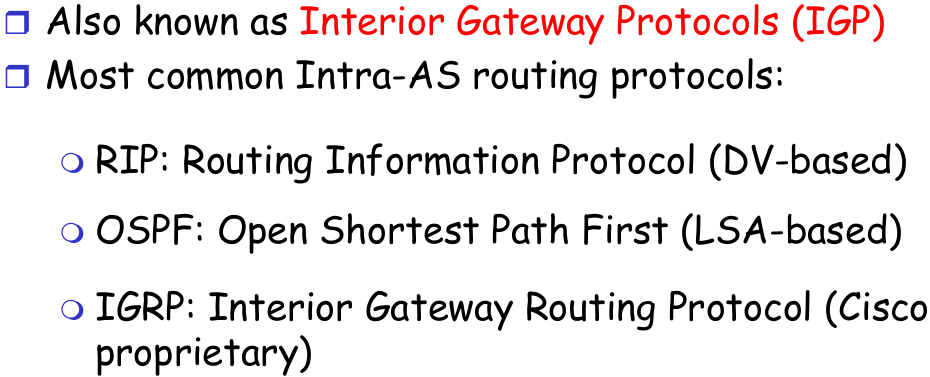
\includegraphics[width=0.49\textwidth]{ip_intra}
  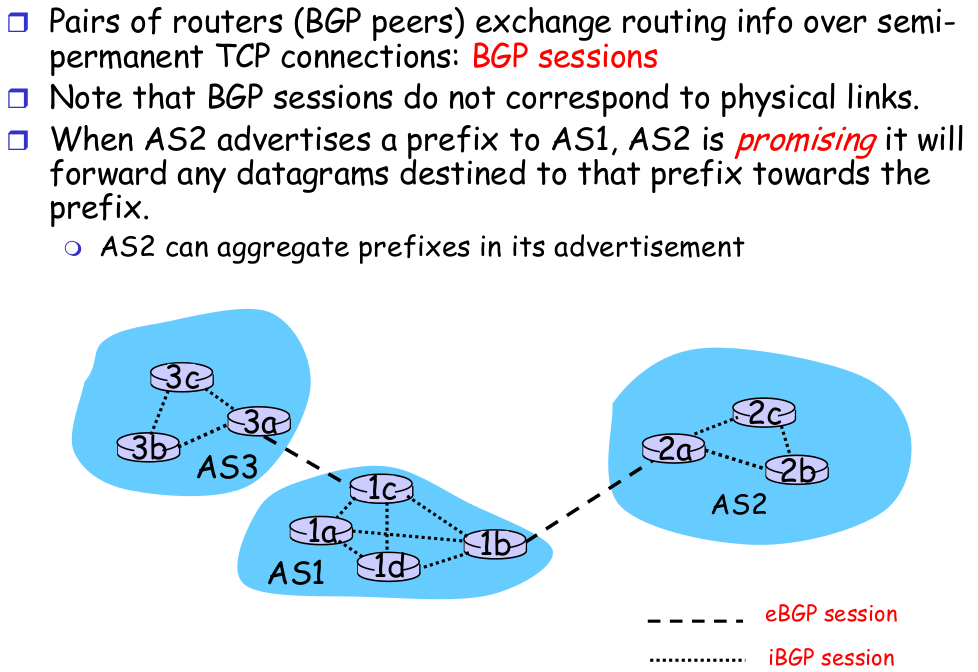
\includegraphics[width=0.49\textwidth]{ip_bgp}
\end{figure}

\key{Why different Intra- and Inter-AS routing ?}
\begin{figure}[H]
  \centering
  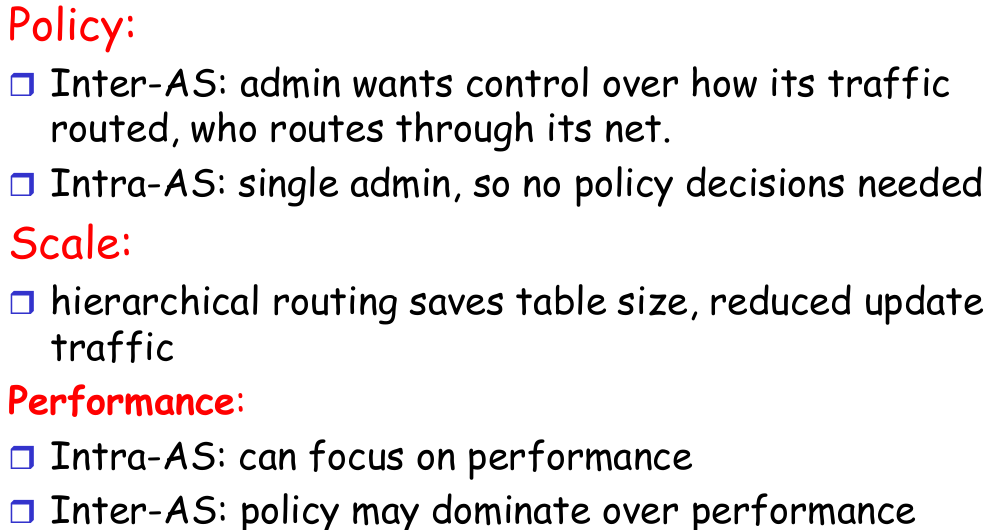
\includegraphics[width=0.5\textwidth]{ip_intra_vs_inter}
\end{figure}

\subsection{Broadcast and multicast routing}

\key{Multicast Routing}
\begin{figure}[H]
  \centering
  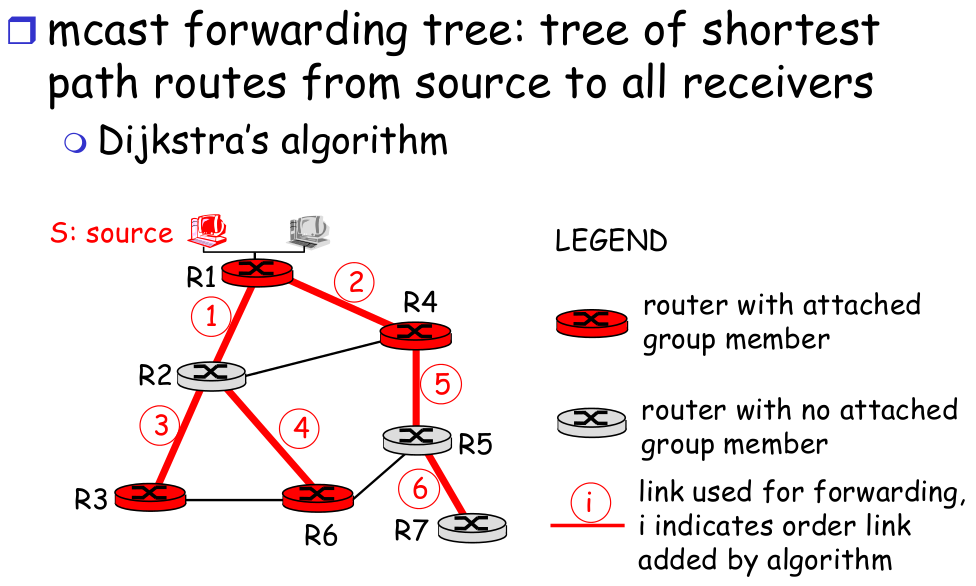
\includegraphics[width=0.49\textwidth]{source_based}
  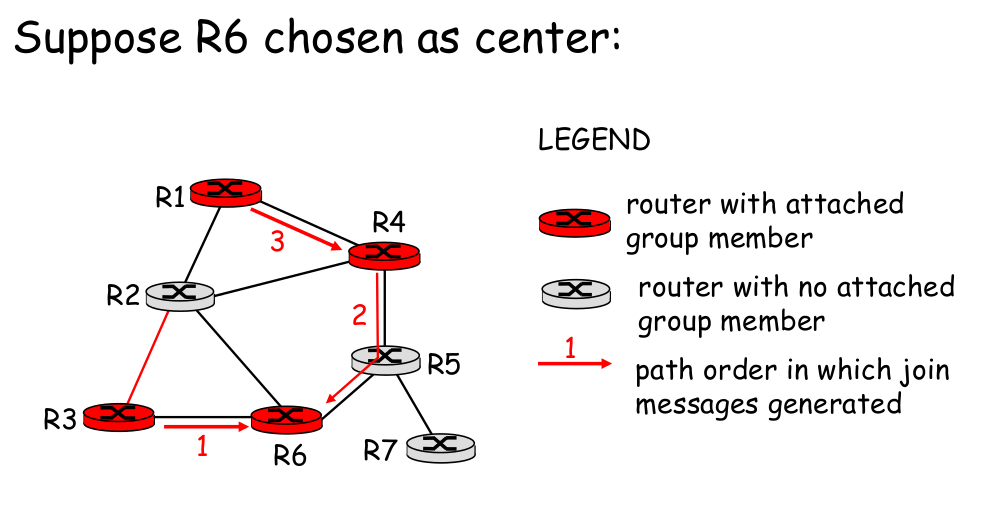
\includegraphics[width=0.49\textwidth]{center_based}
\end{figure}

\section{Link Layer}

\subsection{Introduction and services}

\key{Link Layer Services}
\begin{figure}[H]
  \centering
  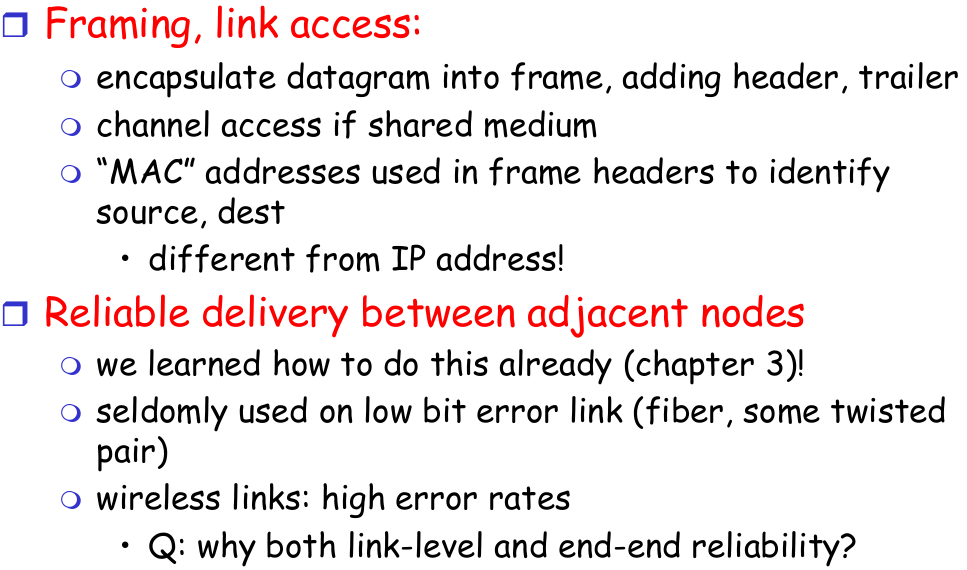
\includegraphics[width=0.48\textwidth]{link_services1}
  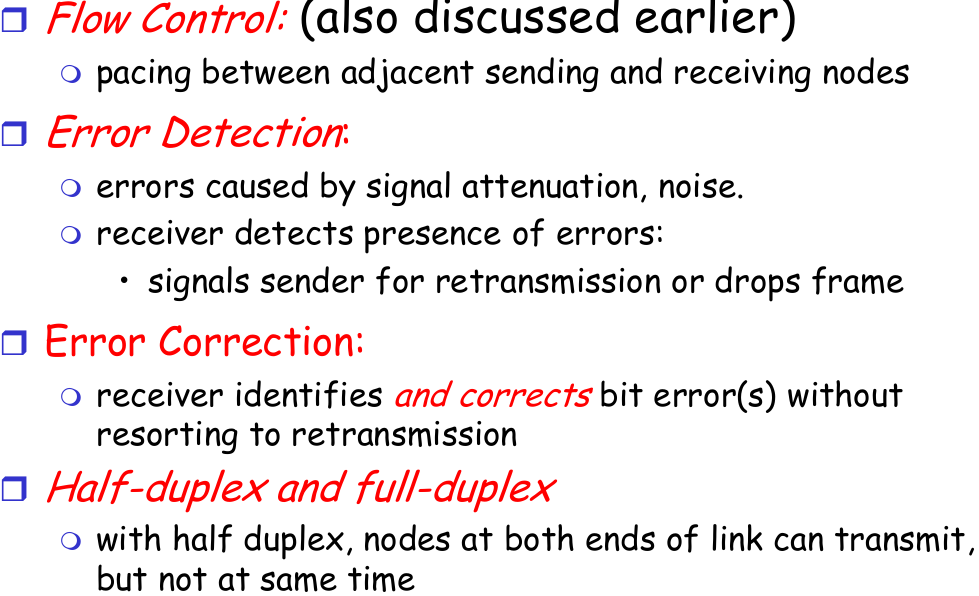
\includegraphics[width=0.48\textwidth]{link_services2}
\end{figure}

\subsection{Error detection and correction}

\key{Hamming distance} The (min) number of bits that differ, that is, need to
be flipped/inverted to change from one codeword to the other.

If the minimum Hamming distance between any two valid codewords is $d$ , then
detect any error up to $d-1$ bits, and can correct any error up to $(d-1)/2$ (if
$d$ is odd), or $d/2-1$ (if $d$ is even) bits.

\key{Checksumming: Cyclic Redundancy Check}
\begin{figure}[H]
  \centering
  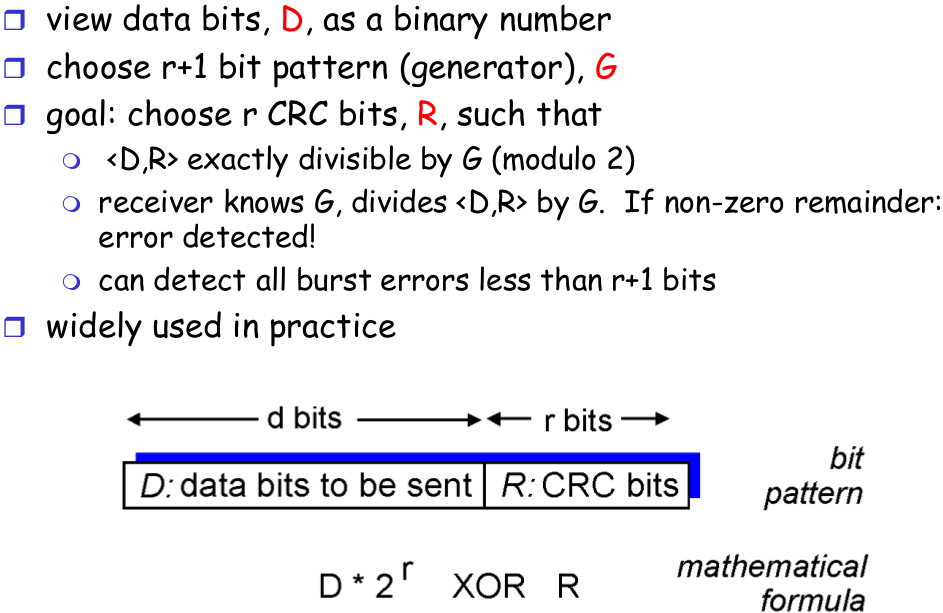
\includegraphics[width=0.48\textwidth]{crc}
  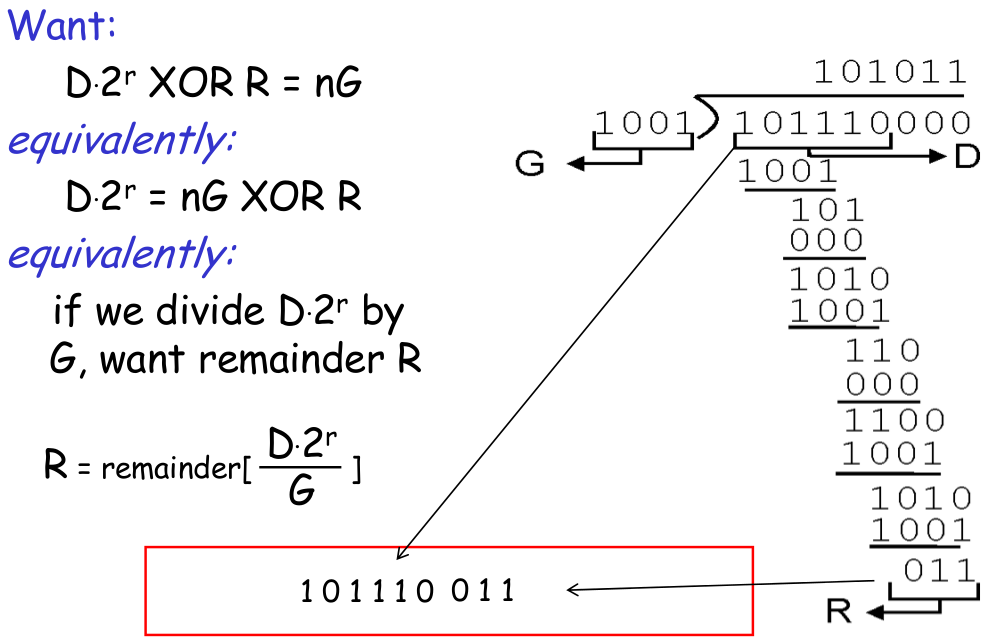
\includegraphics[width=0.48\textwidth]{crc_example}
\end{figure}

\subsection{Multiple access protocols}

\key{MAC Protocols: a taxonomy}
\begin{figure}[H]
  \centering
  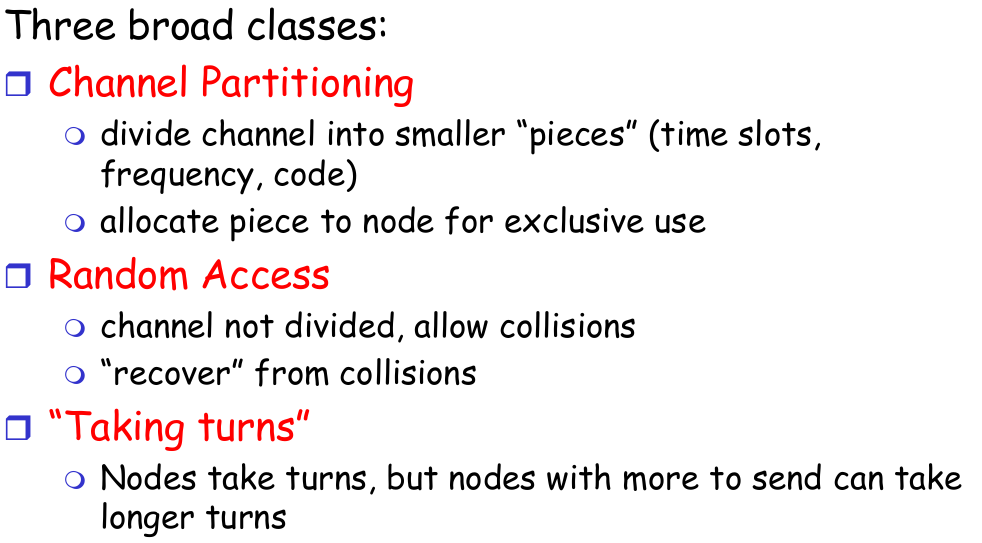
\includegraphics[width=0.48\textwidth]{mac}
\end{figure}

\key{Slotted ALOHA}
\begin{figure}[H]
  \centering
  \includegraphics[width=0.48\textwidth]{slotted_aloha}
  \includegraphics[width=0.48\textwidth]{slotted_aloha_p}
\end{figure}

\key{Pure (unslotted) ALOHA}
\begin{figure}[H]
  \centering
  \includegraphics[width=0.48\textwidth]{pure_aloha}
  \includegraphics[width=0.48\textwidth]{pure_aloha_p}
\end{figure}

\key{CSMA (Carrier Sense Multiple Access)}
\begin{figure}[H]
  \centering
  \includegraphics[width=0.48\textwidth]{csma1}
  \includegraphics[width=0.48\textwidth]{csma2}
\end{figure}

\key{CSMA/CD Collision Detection Delay}
\begin{figure}[H]
  \centering
  \includegraphics[width=0.48\textwidth]{csma_cd}
  \includegraphics[width=0.48\textwidth]{csma_cd_delay}
\end{figure}

\key{Taking Turns MAC protocols}
\begin{figure}[H]
  \centering
  \includegraphics[width=0.48\textwidth]{take_turns}
  \includegraphics[width=0.48\textwidth]{adaptive_tree}
\end{figure}

\subsection{Link-Layer Addressing}


\key{MAC (or LAN or physical or Ethernet) address} used to get datagram from one interface to
another physically-connected interface (same network)

\key{ARP: Address Resolution Protocol}
\begin{figure}[H]
  \centering
  \includegraphics[width=0.48\textwidth]{arp2}
  \includegraphics[width=0.48\textwidth]{arp}
\end{figure}

\key{Routing to another LAN}
\begin{figure}[H]
  \centering
  \includegraphics[width=0.48\textwidth]{arp_other_lan}
  \includegraphics[width=0.48\textwidth]{arp_other_lan2}
\end{figure}

\subsection{Ethernet}

\key{Ethernet Frame Structure}
\begin{figure}[H]
  \centering
  \includegraphics[width=0.48\textwidth]{eth_frame1}
  \includegraphics[width=0.48\textwidth]{eth_frame2}
\end{figure}

\key{Ethernet CSMA/CD algorithm}
\begin{figure}[H]
  \centering
  \includegraphics[width=0.48\textwidth]{eth_csma1}
  \includegraphics[width=0.48\textwidth]{eth_csma2}
\end{figure}

\key{CSMA/CD efficiency}
\begin{figure}[H]
  \centering
  \includegraphics[width=0.48\textwidth]{csma_cd_eff1}
  \includegraphics[width=0.48\textwidth]{csma_cd_eff2}
\end{figure}

\key{802.3 Ethernet Standards: Link \& Physical Layers}
\begin{figure}[H]
  \centering
  \includegraphics[width=0.48\textwidth]{802_3}
\end{figure}

\subsection{Interconnections: Hubs and switches}

\key{Hubs and Switches}
\begin{figure}[H]
  \centering
  \includegraphics[width=0.48\textwidth]{hub}
  \includegraphics[width=0.48\textwidth]{switch}
\end{figure}

\key{Switch: frame filtering/forwarding}
\begin{figure}[H]
  \centering
  \includegraphics[width=0.48\textwidth]{switch_table}
  \includegraphics[width=0.48\textwidth]{switch_table2}
\end{figure}

\key{Switches vs. Routers}
\begin{figure}[H]
  \centering
  \includegraphics[width=0.48\textwidth]{switch_vs_router}
\end{figure}

\key{VLANs}
\begin{figure}[H]
  \centering
  \includegraphics[width=0.48\textwidth]{vlan1}
  \includegraphics[width=0.48\textwidth]{vlan2}
\end{figure}

\subsection{MPLS}

\key{Multiprotocol label switching (MPLS)}
\begin{figure}[H]
  \centering
  \includegraphics[width=0.48\textwidth]{mpls1}
  \includegraphics[width=0.48\textwidth]{mpls2}
\end{figure}

\subsection{A day in the life}
\begin{figure}[H]
  \centering
  \includegraphics[width=0.48\textwidth]{day1}
  \includegraphics[width=0.48\textwidth]{day2}
  \includegraphics[width=0.48\textwidth]{day3}
  \includegraphics[width=0.48\textwidth]{day4}
  \includegraphics[width=0.48\textwidth]{day5}
  \includegraphics[width=0.48\textwidth]{day6}
\end{figure}

\section{Wireless and Mobile Networks}


\subsection{Introduction}


\subsection{Wireless Links Characteristics}

\key{Wireless Link Characteristics}
\begin{figure}[H]
  \centering
  \includegraphics[width=0.48\textwidth]{wireless_char}
  \includegraphics[width=0.48\textwidth]{wireless_char2}
\end{figure}

\subsection{IEEE 802.11 Wireless LANs (wifi)}

\key{IEEE 802.11: Multiple Access}
\begin{figure}[H]
  \centering
  \includegraphics[width=0.48\textwidth]{csma_ca1}
\end{figure}

\key{Collision Avoidance: RTS-CTS exchange}
\begin{figure}[H]
  \centering
  \includegraphics[width=0.48\textwidth]{rts_cts1}
  \includegraphics[width=0.48\textwidth]{rts_cts2}
\end{figure}

\key{802.11 frame: addressing}
\begin{figure}[H]
  \centering
  \includegraphics[width=0.48\textwidth]{802_11_addr}
  \includegraphics[width=0.48\textwidth]{802_11_addr2}
\end{figure}

\key{802.11: advanced capabilities}
\begin{figure}[H]
  \centering
  \includegraphics[width=0.48\textwidth]{802_11_adv}
  \includegraphics[width=0.48\textwidth]{802_11_adv2}
\end{figure}

\subsection{Cellular Internet Access}

\subsection{Principles: addressing and routing to mobile users}

\subsection{Mobile IP}

\key{GSM: handoff with common MSC}
\begin{figure}[H]
  \centering
  \includegraphics[width=0.48\textwidth]{gsm_handoff}
\end{figure}



\key{Mobility: GSM versus Mobile IP}
\begin{figure}[H]
  \centering
  \includegraphics[width=0.48\textwidth]{gsm_vs_mobileip}
\end{figure}






\section{Multimedia and Quality of Service}

\subsection{Multimedia Networking Applications}

\key{MM Networking Applications}
\begin{figure}[H]
  \centering
  \includegraphics[width=0.48\textwidth]{mm_app}
\end{figure}

\subsection{Streaming stored audio and video}

\key{RTSP: out of band control}
\begin{figure}[H]
  \centering
  \includegraphics[width=0.48\textwidth]{rtsp1}
  \includegraphics[width=0.48\textwidth]{rtsp2}
\end{figure}

\key{Internet Phone: Packet Loss and Delay}
\begin{figure}[H]
  \centering
  \includegraphics[width=0.48\textwidth]{loss1}
  \includegraphics[width=0.48\textwidth]{loss2}
\end{figure}

\key{Recovery from packet loss}
\begin{figure}[H]
  \centering
  \includegraphics[width=0.48\textwidth]{recovery1}
  \includegraphics[width=0.48\textwidth]{recovery2}
\end{figure}

\subsection{Protocols for real-time interactive applications}

\key{Real-Time Protocol (RTP)}
\begin{figure}[H]
  \centering
  \includegraphics[width=0.48\textwidth]{rtp1}
  \includegraphics[width=0.48\textwidth]{rtp2}
\end{figure}

\key{Real-Time Control Protocol (RTCP)}
\begin{figure}[H]
  \centering
  \includegraphics[width=0.48\textwidth]{rtcp1}
  \includegraphics[width=0.48\textwidth]{rtcp2}
\end{figure}

\key{SIP: Session Initiation Protocol}
\begin{figure}[H]
  \centering
  \includegraphics[width=0.48\textwidth]{sip1}
  \includegraphics[width=0.48\textwidth]{sip2}
\end{figure}

\subsection{Providing multiple classes of service}

\key{Policing Mechanisms}
\begin{figure}[H]
  \centering
  \includegraphics[width=0.48\textwidth]{bucket1}
  \includegraphics[width=0.48\textwidth]{bucket2}
\end{figure}

\key{Call Admission}
\begin{figure}[H]
  \centering
  \includegraphics[width=0.48\textwidth]{rsvp1}
  \includegraphics[width=0.48\textwidth]{rsvp2}
\end{figure}







\section{Network Security}

\subsection{What is network security?}
\key{What is network security?}
\begin{figure}[H]
  \centering
  \includegraphics[width=0.48\textwidth]{sec}
\end{figure}

\subsection{Principles of cryptography}

\key{Symmetric vs. Public  key cryptography}
\begin{figure}[H]
  \centering
  \includegraphics[width=0.48\textwidth]{symmetric}
  \includegraphics[width=0.48\textwidth]{public}
\end{figure}

\key{RSA: Choosing keys}
\begin{figure}[H]
  \centering
  \includegraphics[width=0.48\textwidth]{rsa1}
  \includegraphics[width=0.48\textwidth]{rsa2}
\end{figure}

\key{RSA: another important property}
\begin{figure}[H]
  \centering
  \includegraphics[width=0.48\textwidth]{rsa_property}
\end{figure}

\subsection{Message integrity}

\key{Message Digests}
\begin{figure}[H]
  \centering
  \includegraphics[width=0.48\textwidth]{hash1}
  \includegraphics[width=0.48\textwidth]{hash2}
\end{figure}

\key{Digital Signatures}
\begin{figure}[H]
  \centering
  \includegraphics[width=0.48\textwidth]{sig1}
  \includegraphics[width=0.48\textwidth]{sig2}
\end{figure}

\key{Certification Authorities}
\begin{figure}[H]
  \centering
  \includegraphics[width=0.48\textwidth]{ca1}
  \includegraphics[width=0.48\textwidth]{ca2}
\end{figure}

\subsection{Securing e-mail}

\key{PGP}
\begin{figure}[H]
  \centering
  \includegraphics[width=0.48\textwidth]{pgp}
\end{figure}


\end{document}
